\chapter{Analysis}
\section*{Overview}
This section introduces the background for the EEW system in place in Japan, consisting of EEW Forecasts and EEW Warnings, and together with the tsunami warnings. Concepts such as intensities, magnitude and epicentres are defined. Two key users and targets are identified, specifically passionate geologists and earthquake-sensitive industries, each having different requirements. A client in the former was interviewed, together with a thorough analysis and comparison of some existing solutions such as SREV, JQuake, KEVI and Quarog. A detailed requirement specification and the critical path is also outlined, consisting of DM-D.S.S. parsing, real-time monitoring, past-earthquake viewing and joint functionalities.

\section{Background Information}

\subsection{The Early Earthquake Warning System}

Earthquake is one of the most common natural disasters in the whole world, and direct consequences of earthquakes include tsunamis which could be catastrophic.

Japan, sitting on the intersection of the Eurasian, the Philippine and the North-American plates, is the countries with most earthquakes. Historically, the Great Kant\=o Earthquake (関東大震災) in 1923, the Great East Japan Earthquake (東日本大震災) in 2011 (a.k.a. the T\=ohoku Earthquake) and the recent 2024 Noto Peninsula Earthquake (能登半島地震) all caused hundreds of deaths, both due to the result of the earthquake(s) and the resulting tsunami.

To provide protection to its residents, the \href{https://www.jma.go.jp/jma/index.html}{Japan Meteorological Agency} (JMA, 気象庁), together with the \href{https://www.bosai.go.jp}{National Research Institute for Earth Science and Disaster Resilience (NIED, 防災科研)} placed thousands of \textbf{earthquake sensors} across Japan (the Hi-net, the K-NET, the KiK-net and the F-NET), with several of them lying deep in the sea bed, measuring displacement, velocity and acceleration, which are connected to multiple servers, including two located in \=Osaka and T\=okyo.

Using data obtained from the sensors, computers do some complicated algorithms (mentioned below) to send out \textbf{early earthquake warnings (EEWs, 緊急地震速報)} automatically within milliseconds. There are two types of EEWs:
\begin{enumerate}
    \item \textbf{EEW (Forecast, 予報).} Sent out to \textbf{highly-dependent industries} (e.g. rail industry, power plants) and \textbf{subscribed users}, when maximum intensity level of more than 3, or a magnitude of more than 3.5 is expected.
    \item \textbf{EEW (Warning, 警報).} Sent out to \textbf{everyone} via TV, Radio, Mobile Phone, SMS, etc., when a maximum intensity level of more than 4 is expected.
\end{enumerate}

After the earthquake, JMA staff will determine the location and severity of tsunami warnings to be issued, if necessary.

\subsection{Earthquake Terminology}

\begin{itemize}
    \item \textbf{Intensity (震度).} The intensity describes the intensity vibration of a point due to an earthquake. It is not unique to an earthquake - \textbf{different places can have different intensities} due to the distance to the epicentre, and intensity will also change over time. JMA measures intensity using \textbf{9 levels: 1, 2, 3, 4, 5--, 5+, 6--, 6+ and 7} in increasing order.
    \item \textbf{Magnitude/Scale.} The magnitude of an earthquake describes the energy released in the earthquake in a logarithmic scale. \textbf{It is unique to an earthquake.}
    \item \textbf{Epicentre/Hypocentre.} The epicentre is the surface point directly above the true centre of the earthquake.
    \item \textbf{Focal Depth.} The focal depth is the depth of the true centre of the earthquake.
    \item \textbf{P-Wave and S-Wave.} These are seismic waves, sourced from the true centre of the earthquake, travelling at different speeds, with Primary (P)-Wave travelling faster and Secondary (S)-Wave travelling slower.
\end{itemize}

\section{Problem Area}
The main goal of this application is to provide a visualisation of the earthquake/tsunami related data feed(s) provided by JMA's affiliated institution, \href{https://dmdata.jp}{Disaster Mitigation Data Send Service (DM-D.S.S)}, and some other data feeds as well. There are numerous apps providing a list of recent earthquakes, the real-time data measured by the sensors, and the real time earthquake warning displayed on a map, but rarely are there good apps that combine all those features together satisfyingly, with just the necessary features the author needs.

Some applications are no longer being updated due to change in the user's policy of the related data feed. Furthermore, most of the apps available are only in Japanese, not in English or my home language Chinese, which can create trouble for the author to understand.

\section{Client and End User}
The primary target of this application will be passionate geographers and geologists who are interested in the study of earthquake observations and predictions. The age group of this vary all the way from primary-school students to adults, including the author who has been amazed by the technology since the age of 12. They could take any employment, ranging from students to full-time jobs. Their proficiency usually varies, since there are people new to this field who probably does not have much knowledge, so the interface of the application should be relatively user-friendly and understandable, hiding unnecessary technical complexities.

Another target client could be industries which highly rely on earthquake predictions due to the risk imposed by earthquakes. High-speed railway and nuclear power plants are good examples of this. Therefore, the staff in charge monitoring will usually have higher proficiency and would like more detailed data of the earthquake. However, they will only need the necessary data from earthquakes happening close to them and only require intensity data of the point in interest (e.g. the power plant). To put this into content, an earthquake happening 1000 km away from them does not need to be fed into their system, while they would like to see the intensity of the shock and the arrival time of the seismic waves to decide the actions. In fact, the author really likes investigating on the rail industry, whose infrastructure could be greatly affected by earthquakes.

\autoref{tab:users} compares relative features of these two target users/clients.

\begin{table}[htp]
    \centering

    \begin{tabular}{c|l|p{0.36\linewidth}}
        Feature              & Primary Target                     & Secondary Target                                     \\
        \hline
        Description          & Passionate Geologists              & Earthquake-Sensitive Industries                      \\
        Age                  & Varies (Middle School -- Adults)   & Work Age                                             \\
        Reason               & Monitor Live \& Latest Earthquakes & Monitor Risks to Infrastructure                      \\
        Proficiency          & Varies (Beginner -- Amateur)       & Trained Professional                                 \\
        General Requirements & Monitor Overall Movement           & Alert intensity and arrival time at certain location \\
    \end{tabular}

    \caption{Comparison of target users and clients}
    \label{tab:users}
\end{table}

\section{Research Methodology}
\subsection{Client Interview}
The author interviewed my friend Wesley Ma, who is a passionate geologist on earthquake studies and also monitor earthquakes regularly.

\begin{enumerate}
    \item \textit{Which earthquake monitoring apps do you use?}

          \textbf{Response:} JQuake, SREV, Quarog, KEVI, Kyoshin-Monitor (Support discontinued), Kiwi Monitor (Support discontinued)

    \item \textit{Do you subscribe/pay to services such as DM-D.S.S. to use earthquake monitoring apps, and do you think it is worth the price?}

          \textbf{Response:} Yes. However, DM-D.S.S. is a little expensive. However, the price becomes more affordable considering the information provided by the subscription.

    \item \textit{Do you watch YouTube livestreams on earthquake monitoring?}

          \textbf{Response:} I do not usually watch the live streams, as almost no one who has already has a monitoring app will use the stream. They provide mostly the same information as the applications, just real-time streaming the windows.

    \item \textit{Why do you use earthquake monitoring apps?}

          \textbf{Response:} To monitor the earthquake. This is derived from my interest in broadcasting culture in Japan. This eventually led me to be intrigued with the development of earthquake monitoring technologies and theories in Japan.

    \item \textit{How often do you use earthquake monitoring apps (e.g. all the time/after school/only after big earthquakes)?}

          \textbf{Response:} After big earthquakes. But I usually open one or two apps for all-day monitoring to catch potential major (or medium) earthquakes.

    \item \textit{Describe the advantages and disadvantages of each of them, mentioning the specific features.}

          \textbf{Response:}
          \begin{itemize}
              \item SREV is a good one, but it is only available in a browser with no app.
              \item Kyoshin-Monitor and Kiwi Monitor are relatively more stable, but the source is not the same as that from the former two apps, and its support is also discontinued.
              \item Quarog has weak response time and interacting interface.
              \item JQuake is the most developed app, which includes nearly all functions that can be thought of. However sometimes the connection of WebSocket is unstable.
              \item KEVI does not have the sound files configured by default. Some information are not displayed clearly enough.
          \end{itemize}

    \item \textit{What features do you use the most/least?}

          \textbf{Response:} Basic earthquake notifications, and should be including sufficient and prompt information.

    \item \textit{What features are redundant in the earthquake monitoring apps you use?}

          \textbf{Response:} KEVI has a weather monitoring function, which could be redundant. But that could be caused by the different purposes of the app. Hence, no further comments. It is not a bad thing.

    \item \textit{What are the critical features of an earthquake monitoring app?}

          \textbf{Response:} To provide accurate, prompt and detailed information according to the source released by the JMA, the information display interface should be easy to read and understand. This is not only helping the people who like to monitor, but more importantly, provides the easiest way to the people who really need to seek information to minimise the harm brought by earthquakes and successive disaster.

    \item \textit{What additional features would you like to have in those existing apps?}

          \textbf{Response:} Summarise all the useful features from different apps into one app. Stable connection. Nothing else.
\end{enumerate}

\subsection{Existing Applications and Solutions}

Based on the applications the author uses and the feedback from interviewee, there are the following commonly-used applications:
\begin{itemize}
    \item JQuake \autocite{soft-jquake};
    \item Scratch Real-time Earthquake Viewer (SREV) \autocite{soft-srev}, which is available in compiled form at \GitHubHref{kotoho7}{scratch-realtime-earthquake-viewer-page} \autocite{soft-srev-github};
    \item Kyoshin EEW Viewer for Ingen (KEVI) \autocite{soft-kevi}, available at \GitHubHref{ingen084}{KyoshinEewViewerIngen} \autocite{soft-kevi-github};
    \item Quarog \autocite{soft-quarog}.
\end{itemize}

\subsubsection{Supported Platforms}

Supported platforms of those apps are listed in \autoref{tab:exist-platform}. In particular, note that SREV is a web-based and GitHub Pages-hosted application therefore supporting all platforms. KEVI is written in .NET Framework and supports the second most platforms, with JQuake not supporting Linux and Quarog only supporting Windows.

\begin{table}[htp]
    \centering
    \begin{tabular}{c|cccc}
        Platform    & JQuake     & SREV       & KEVI       & Quarog     \\
        \hline
        Windows     & \checkmark & \checkmark & \checkmark & \checkmark \\
        macOS       & \checkmark & \checkmark & \checkmark &            \\
        Linux       & \checkmark & \checkmark & \checkmark &            \\
        Android/iOS &            & \checkmark &            &            \\
    \end{tabular}
    \caption{Supported platforms of existing solutions}
    \label{tab:exist-platform}
\end{table}

\subsubsection{Earthquake Monitoring}

An overview feature table of monitoring is included in \autoref{tab:exist-monitoring}. In particular, note that due to the nature of SREV being Scratch-programmed and web-based, it reached a special agreement with DM-D.S.S. to use the API without the need of all users paying for this, since it is hard to integrate such function into a web application.

Quarog is a relatively new application and only supports basic functionalities of EEW Viewing and past earthquake listing, as shown in \autoref{fig:quarog-monitor-features}. JQuake is solely dedicated to earthquake and tsunami monitoring as shown in \autoref{fig:jquake-monitor-features}, while KEVI has features like rain clouds map and natural disaster warning which is beyond the scope of this analysis (which is a burden to users only requiring earthquake monitoring and a waste of storage space).

It is worth noting that for SREV, DM-D.S.S. is integrated with special permission with no login required. For JQuake, although it has tsunami warnings/special warnings, the tsunami forecast is not available, since they use a different data source.

\begin{table}[htp]
    \centering

    \begin{tabular}{c|cccc}
        Feature                        & JQuake     & SREV       & KEVI       & Quarog     \\
        \hline
        NIED Real-time Shake Support   & \checkmark & \checkmark & \checkmark &            \\
        DM-D.S.S. WebSocket Support    & \checkmark & \checkmark & \checkmark & \checkmark \\
        Real-time Sensor Data          & \checkmark & \checkmark & \checkmark &            \\
        Vibration Alert                & \checkmark & \checkmark & \checkmark &            \\
        Past Earthquake List           & \checkmark & \checkmark & \checkmark & \checkmark \\
        Past Earthquake Details        &            & \checkmark & \checkmark & \checkmark \\
        Tsunami Warning                & \checkmark & \checkmark & \checkmark &            \\
        Real-time EEW                  & \checkmark & \checkmark & \checkmark & \checkmark \\
        Calculated Seismic Wavefronts  & \checkmark & \checkmark & \checkmark & \checkmark \\
        User-Defined Key Monitor Point & \checkmark &            & \checkmark &            \\
        Sub-Map for the Okinawa Area   & \checkmark &            & \checkmark &            \\
        Replay                         & \checkmark &            & \checkmark &            \\
    \end{tabular}

    \caption[Feature comparison in monitoring of existing solutions]{Feature comparison in monitoring of existing solutions}
    \label{tab:exist-monitoring}
\end{table}

\begin{figure}[htp]
    \centering

    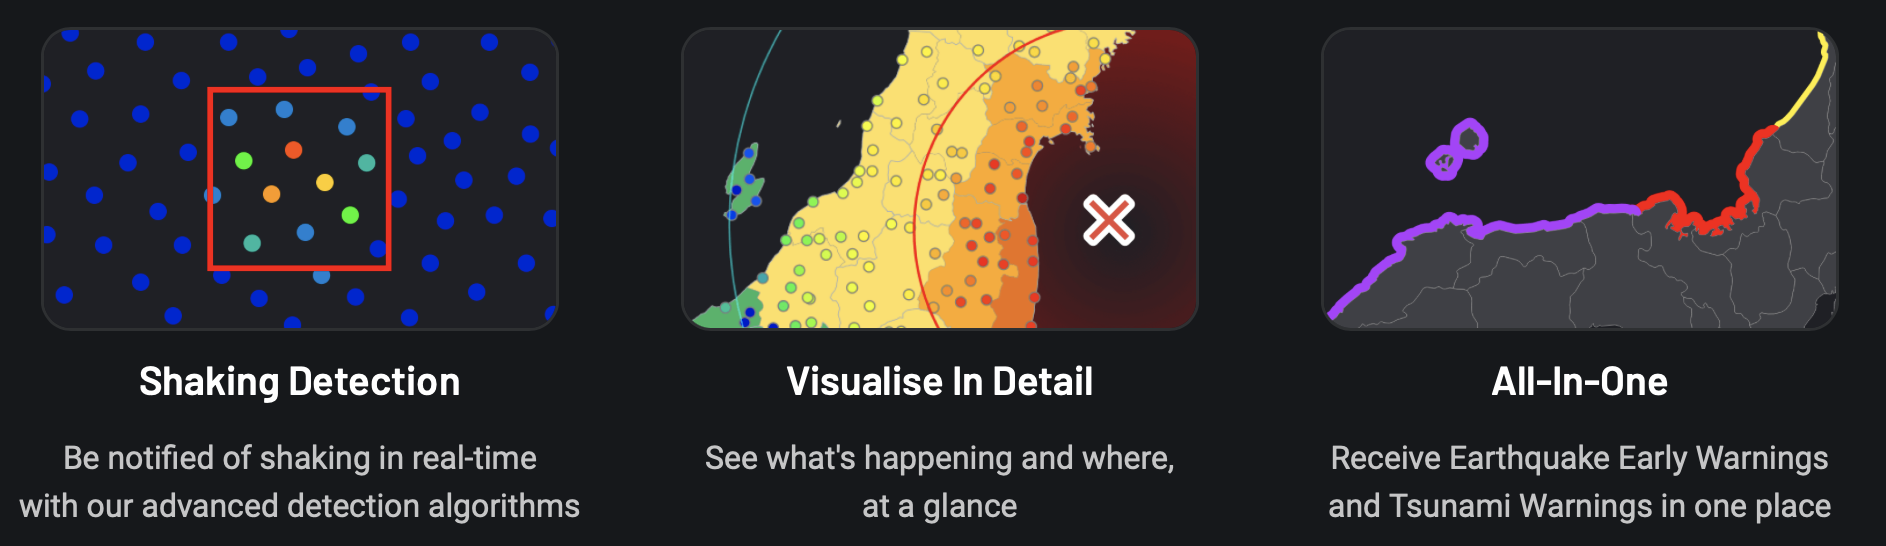
\includegraphics[width=0.6\linewidth]{jquake-features.png}
    \caption[Feature introduction of JQuake]{Feature introduction of JQuake, screenshot from website}
    \label{fig:jquake-monitor-features}
\end{figure}

\begin{figure}[htp]
    \centering

    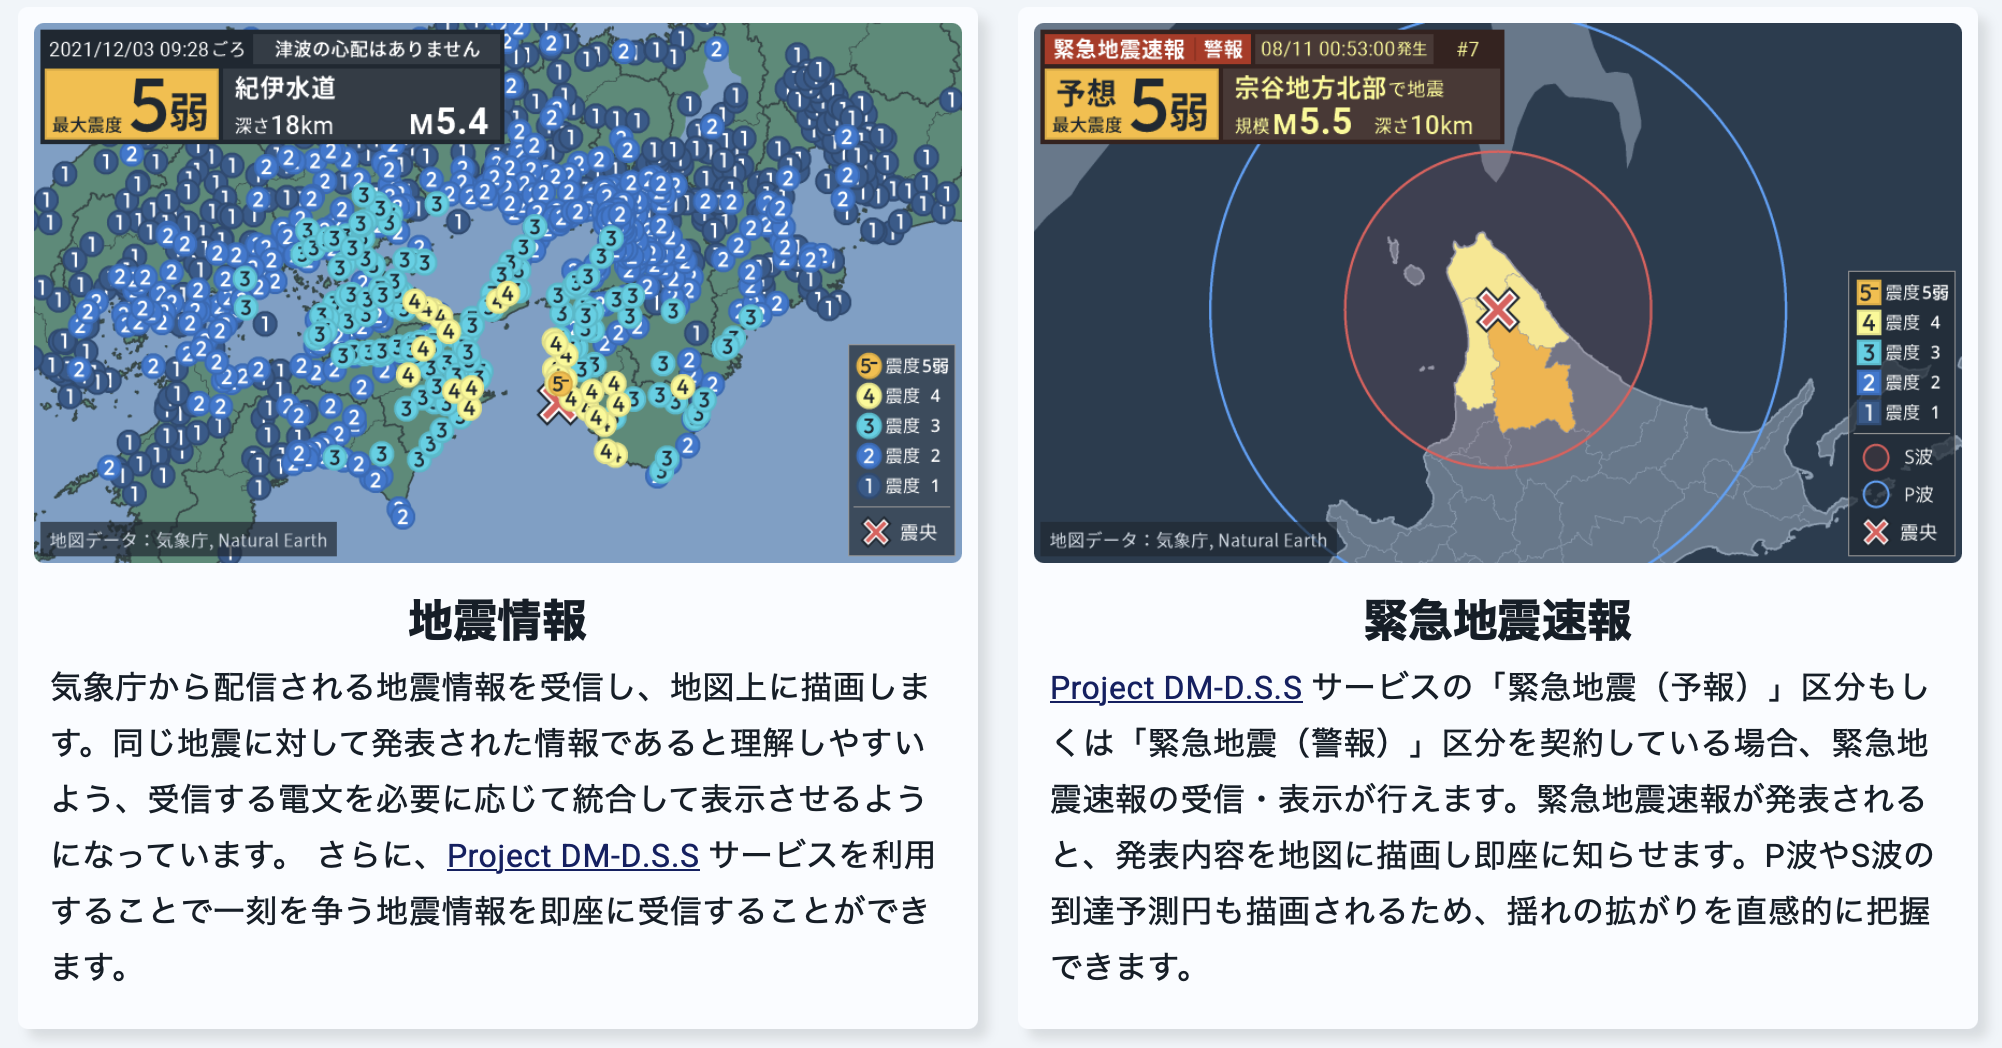
\includegraphics[width=0.6\linewidth]{quarog-features-1.png}\\
    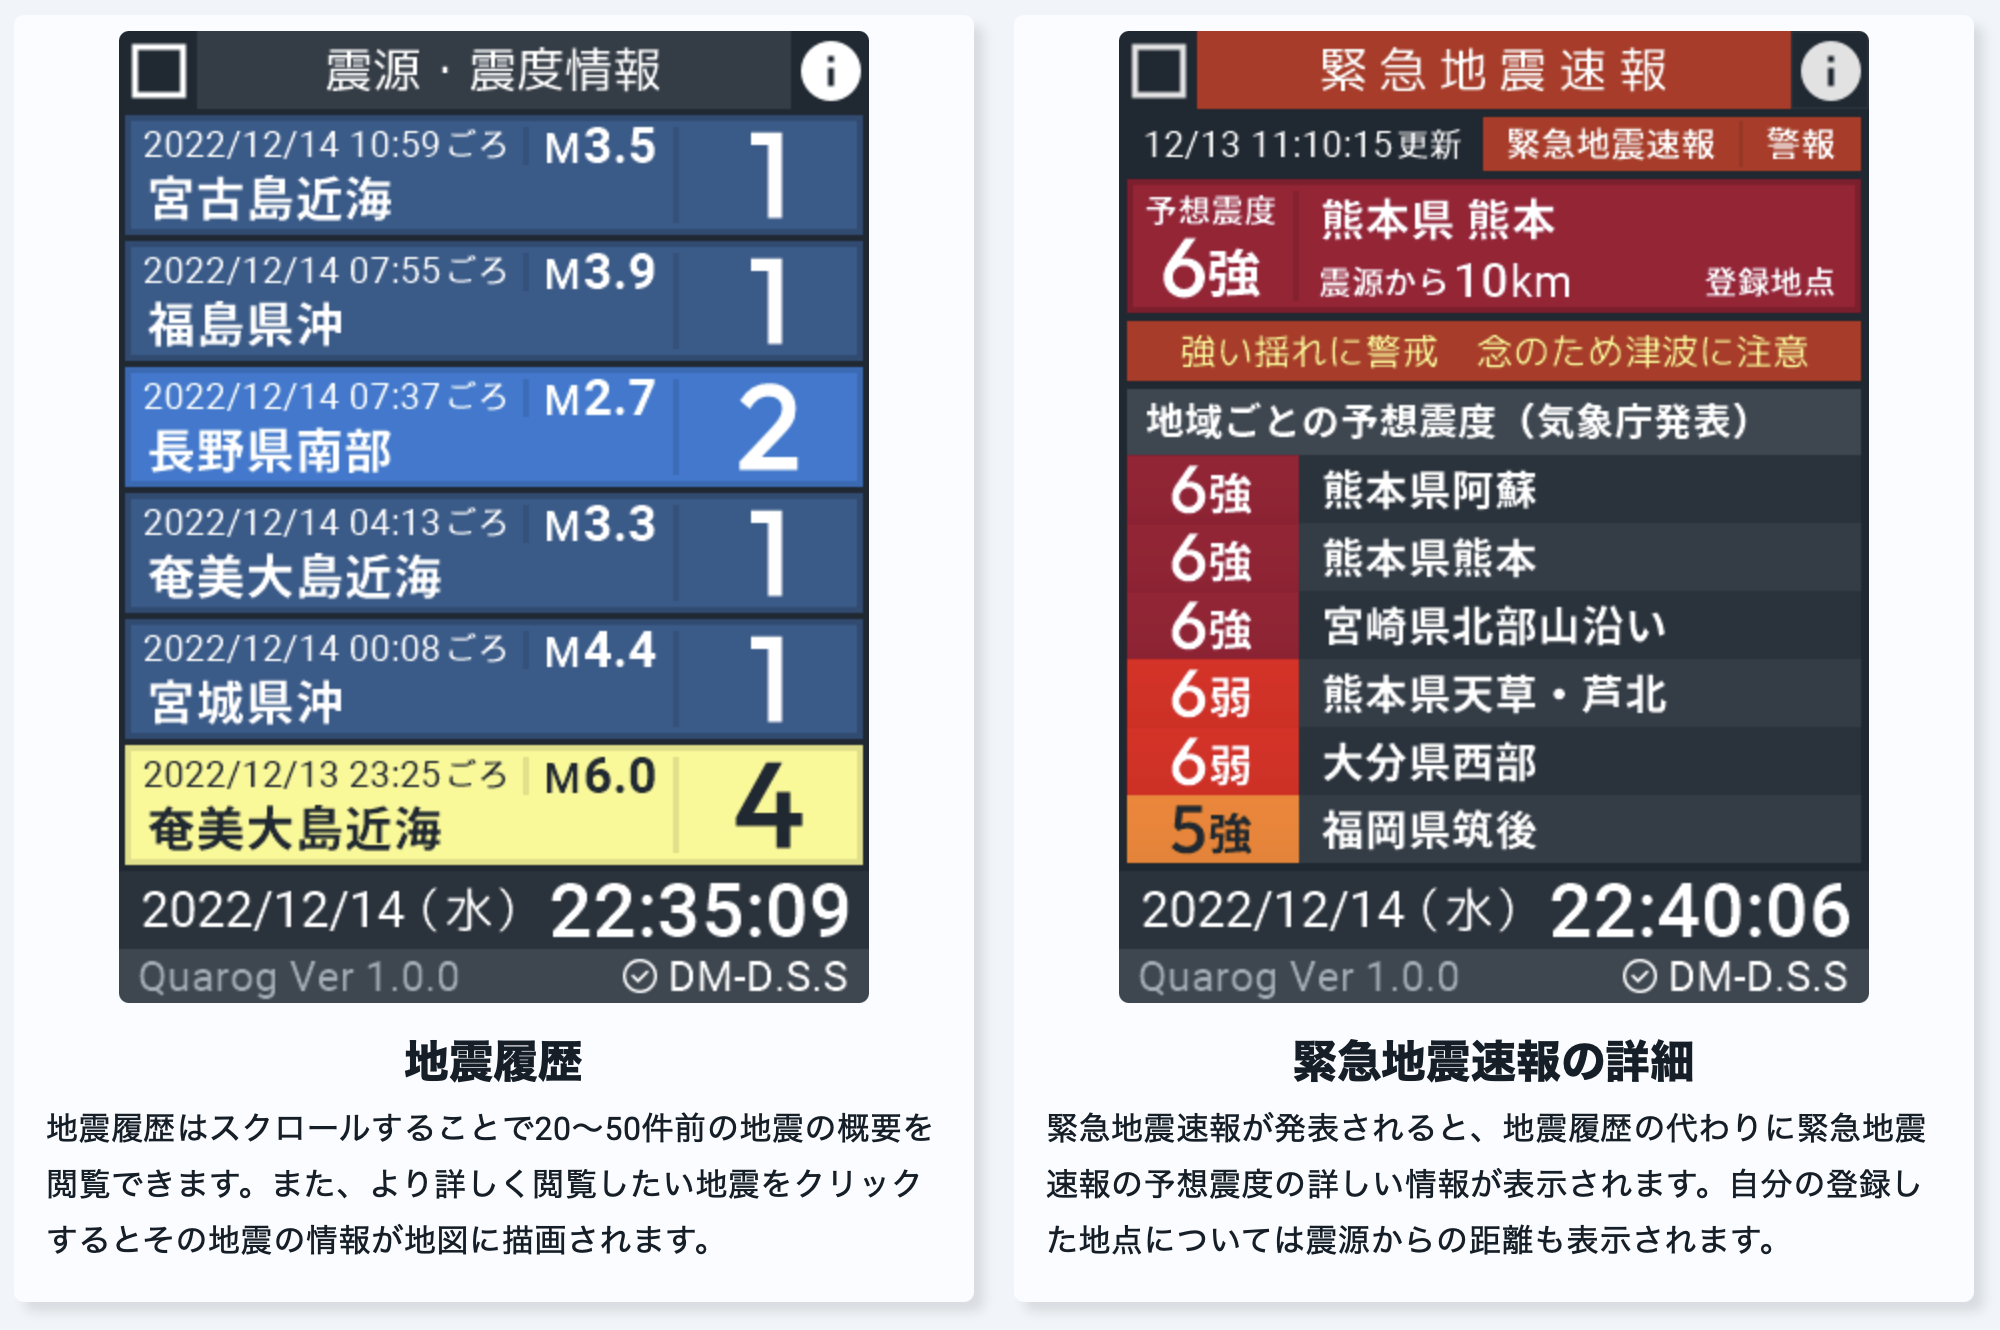
\includegraphics[width=0.6\linewidth]{quarog-features-2.png}
    \caption[Feature introduction of Quarog]{Feature introduction of Quarog, screenshot from website\\
        Top-left: Past earthquake information; Top-right: Real-time EEW;\\
        Bottom-Left: Past earthquake list; Bottom-Right: Details of EEW}
    \label{fig:quarog-monitor-features}
\end{figure}

\subsubsection{Configuration Options}

There are also a variety of configuration options available for all apps, as listed in \autoref{tab:exist-config}. Both KEVI and Quarog supports the adjustment of the colour theme, and Quarog even supports changing the style of how blocks are displayed and coloured as shown in \autoref{fig:kevi-colour-cust} and \autoref{fig:quarog-cust}. Playing a sound on the speaker is also common among the apps to remind the user of earthquakes.

\begin{table}[htp]
    \centering

    \begin{tabular}{c|cccc}
        Feature             & JQuake     & SREV       & KEVI       & Quarog     \\
        \hline
        DM-D.S.S. Login     & \checkmark &            & \checkmark & \checkmark \\
        Sound Alert         & \checkmark & \checkmark & \checkmark & \checkmark \\
        System Notification &            &            & \checkmark &            \\
        Colour Theme        &            &            & \checkmark & \checkmark \\
        Map Colouring Style &            & \checkmark &            & \checkmark \\
    \end{tabular}
    \caption{Feature comparison in configuration and customisability of existing solutions}
    \label{tab:exist-config}
\end{table}

\begin{figure}[htp]
    \centering

    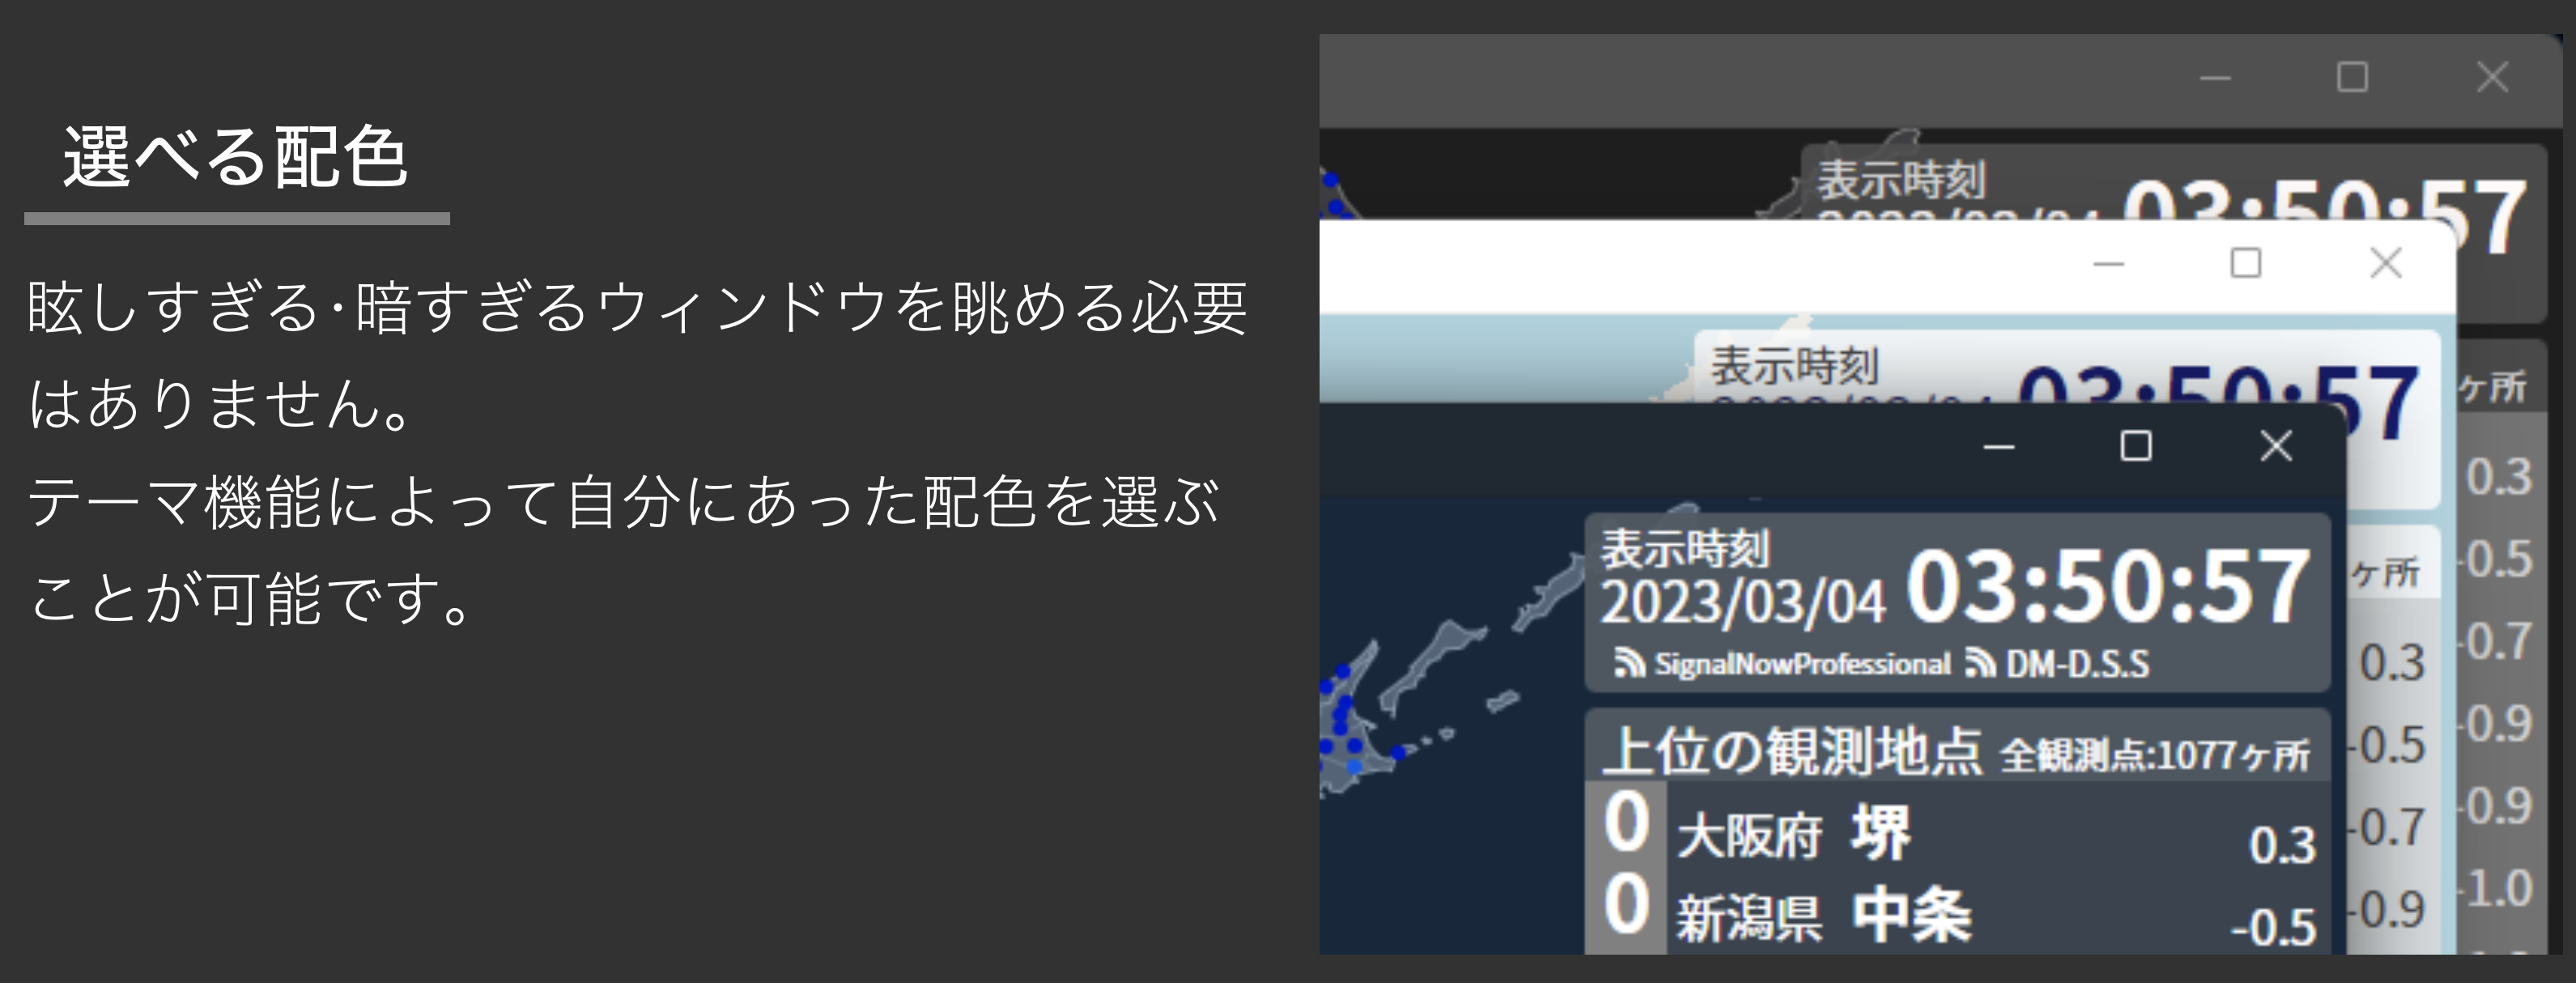
\includegraphics[width=0.5\linewidth]{kevi-colour.png}
    \caption[Customisable colour scheme of KEVI]{Customisable colour scheme of KEVI, screenshot from website}
    \label{fig:kevi-colour-cust}
\end{figure}

\begin{figure}[htp]
    \centering

    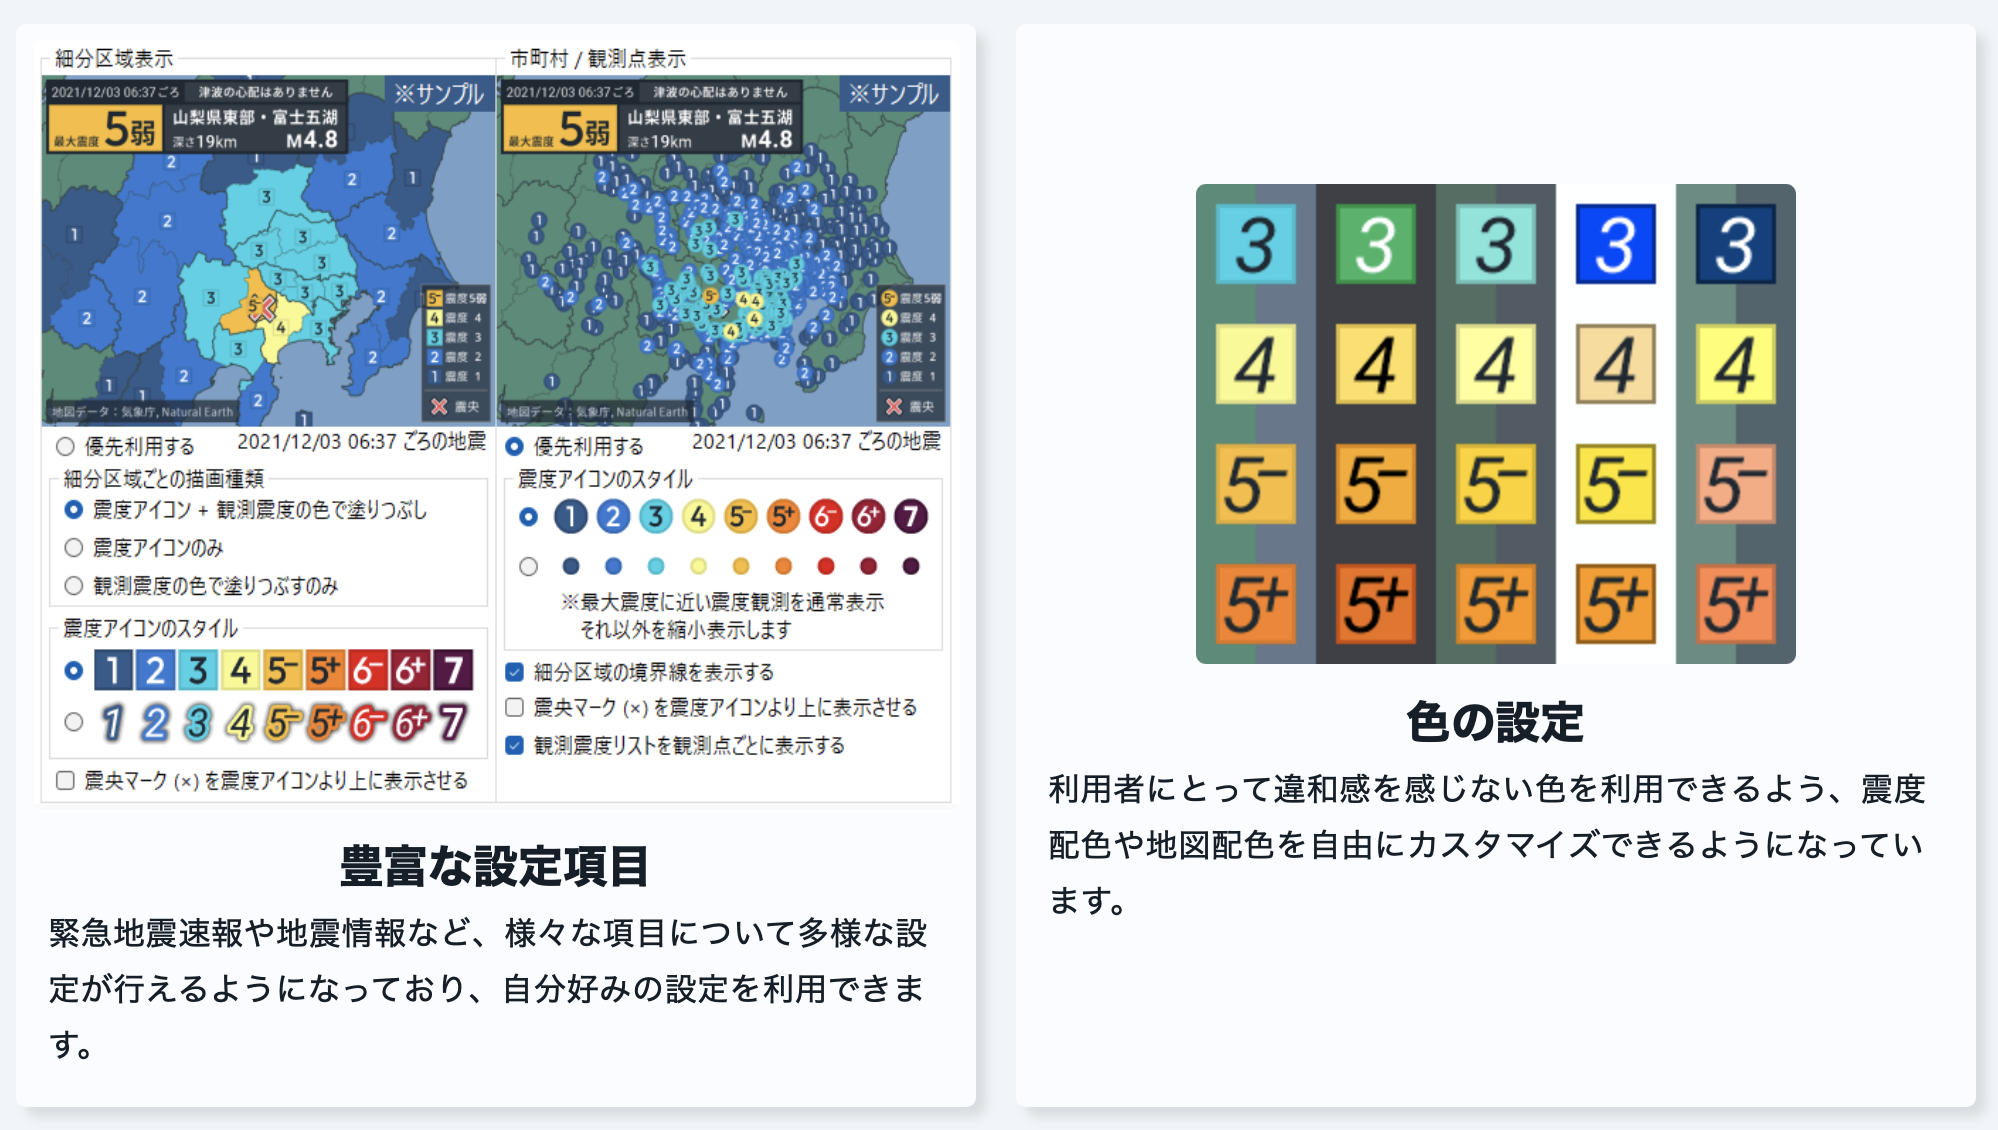
\includegraphics[width=0.6\linewidth]{quarog-cust.png}
    \caption[Customisability of Quarog]{Customisability of Quarog, screenshot from website}
    \label{fig:quarog-cust}
\end{figure}

\subsubsection{GUI Analysis}

All applications are similar in a way, that their past earthquakes list is displayed on a sidebar.

For Quarog and KEVI, an earthquake can be selected from the sidebar to view the details of, as in \autoref{fig:kevi-srev-past-page}. They will both colour on the map the maximum observed intensities by regions. While KEVI chooses to display the regions as colours and also provide an overlay of the observed intensities by observation stations (which will only appear after zoomed in enough, as in \autoref{fig:kevi-map}), Quarog chooses to have a separate button to switch between display of regions, and the display of observation stations.

\begin{figure}[htp]
    \centering

    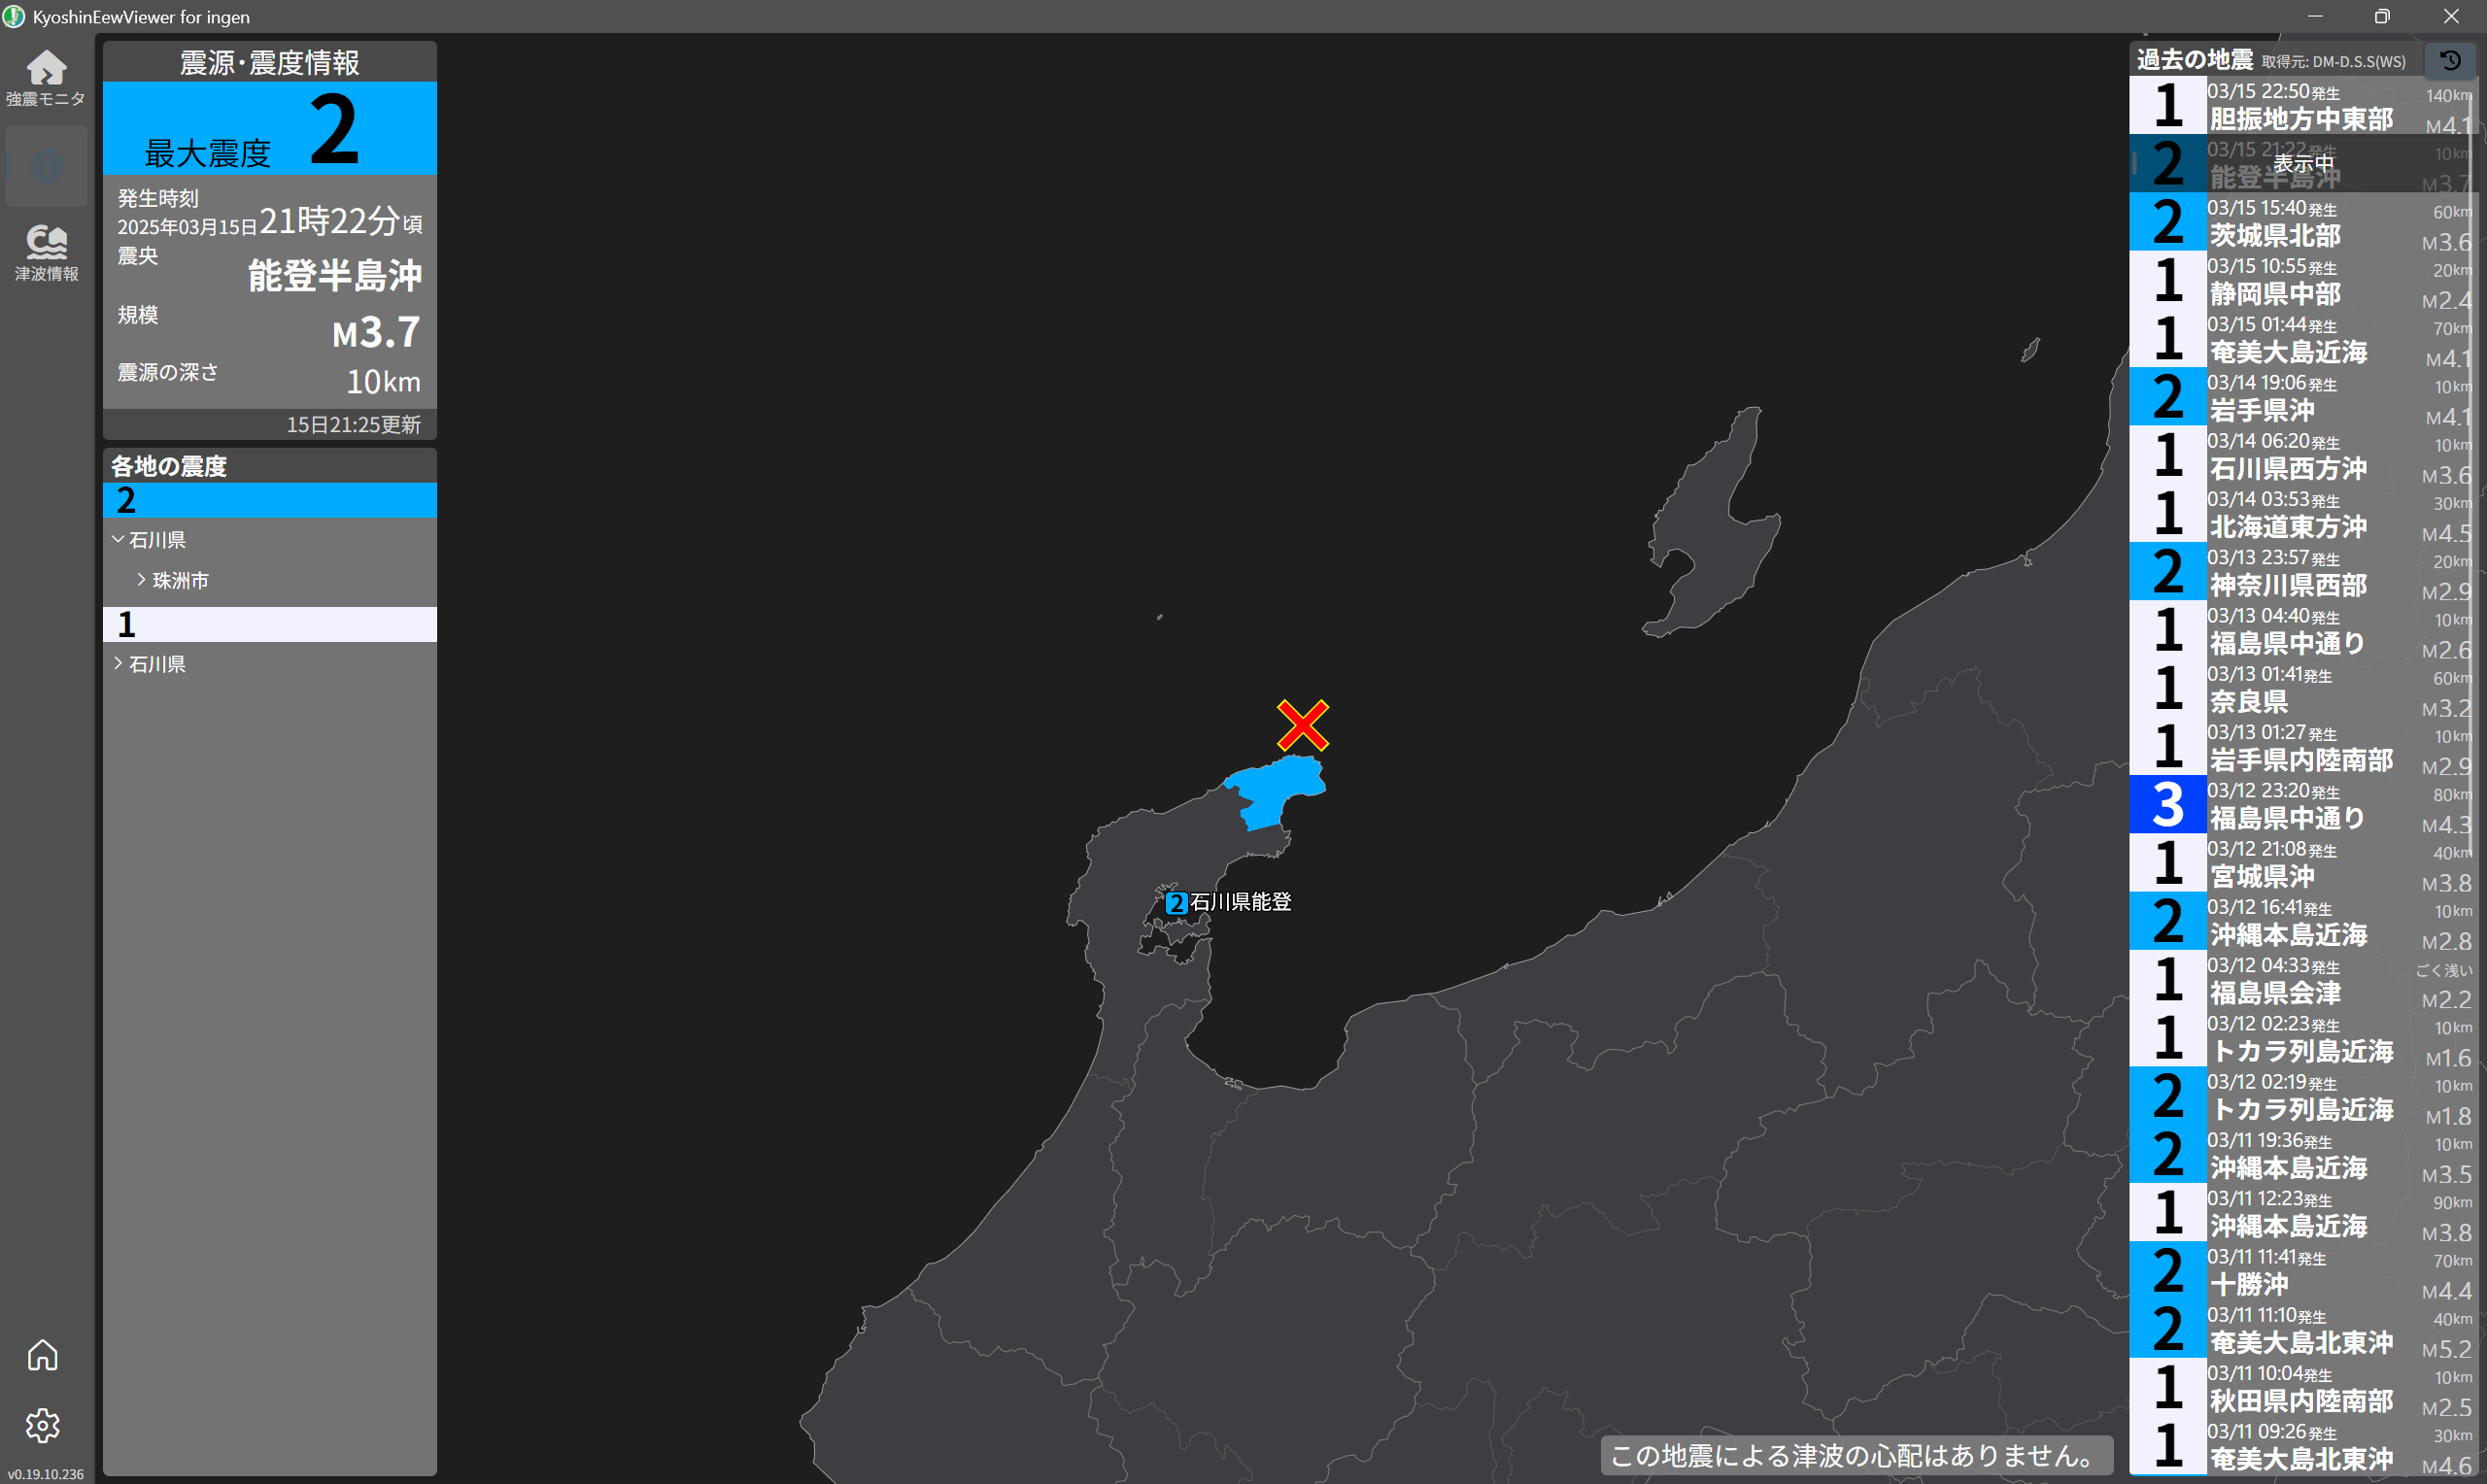
\includegraphics[width=0.7\linewidth]{kevi-past-page.png}
    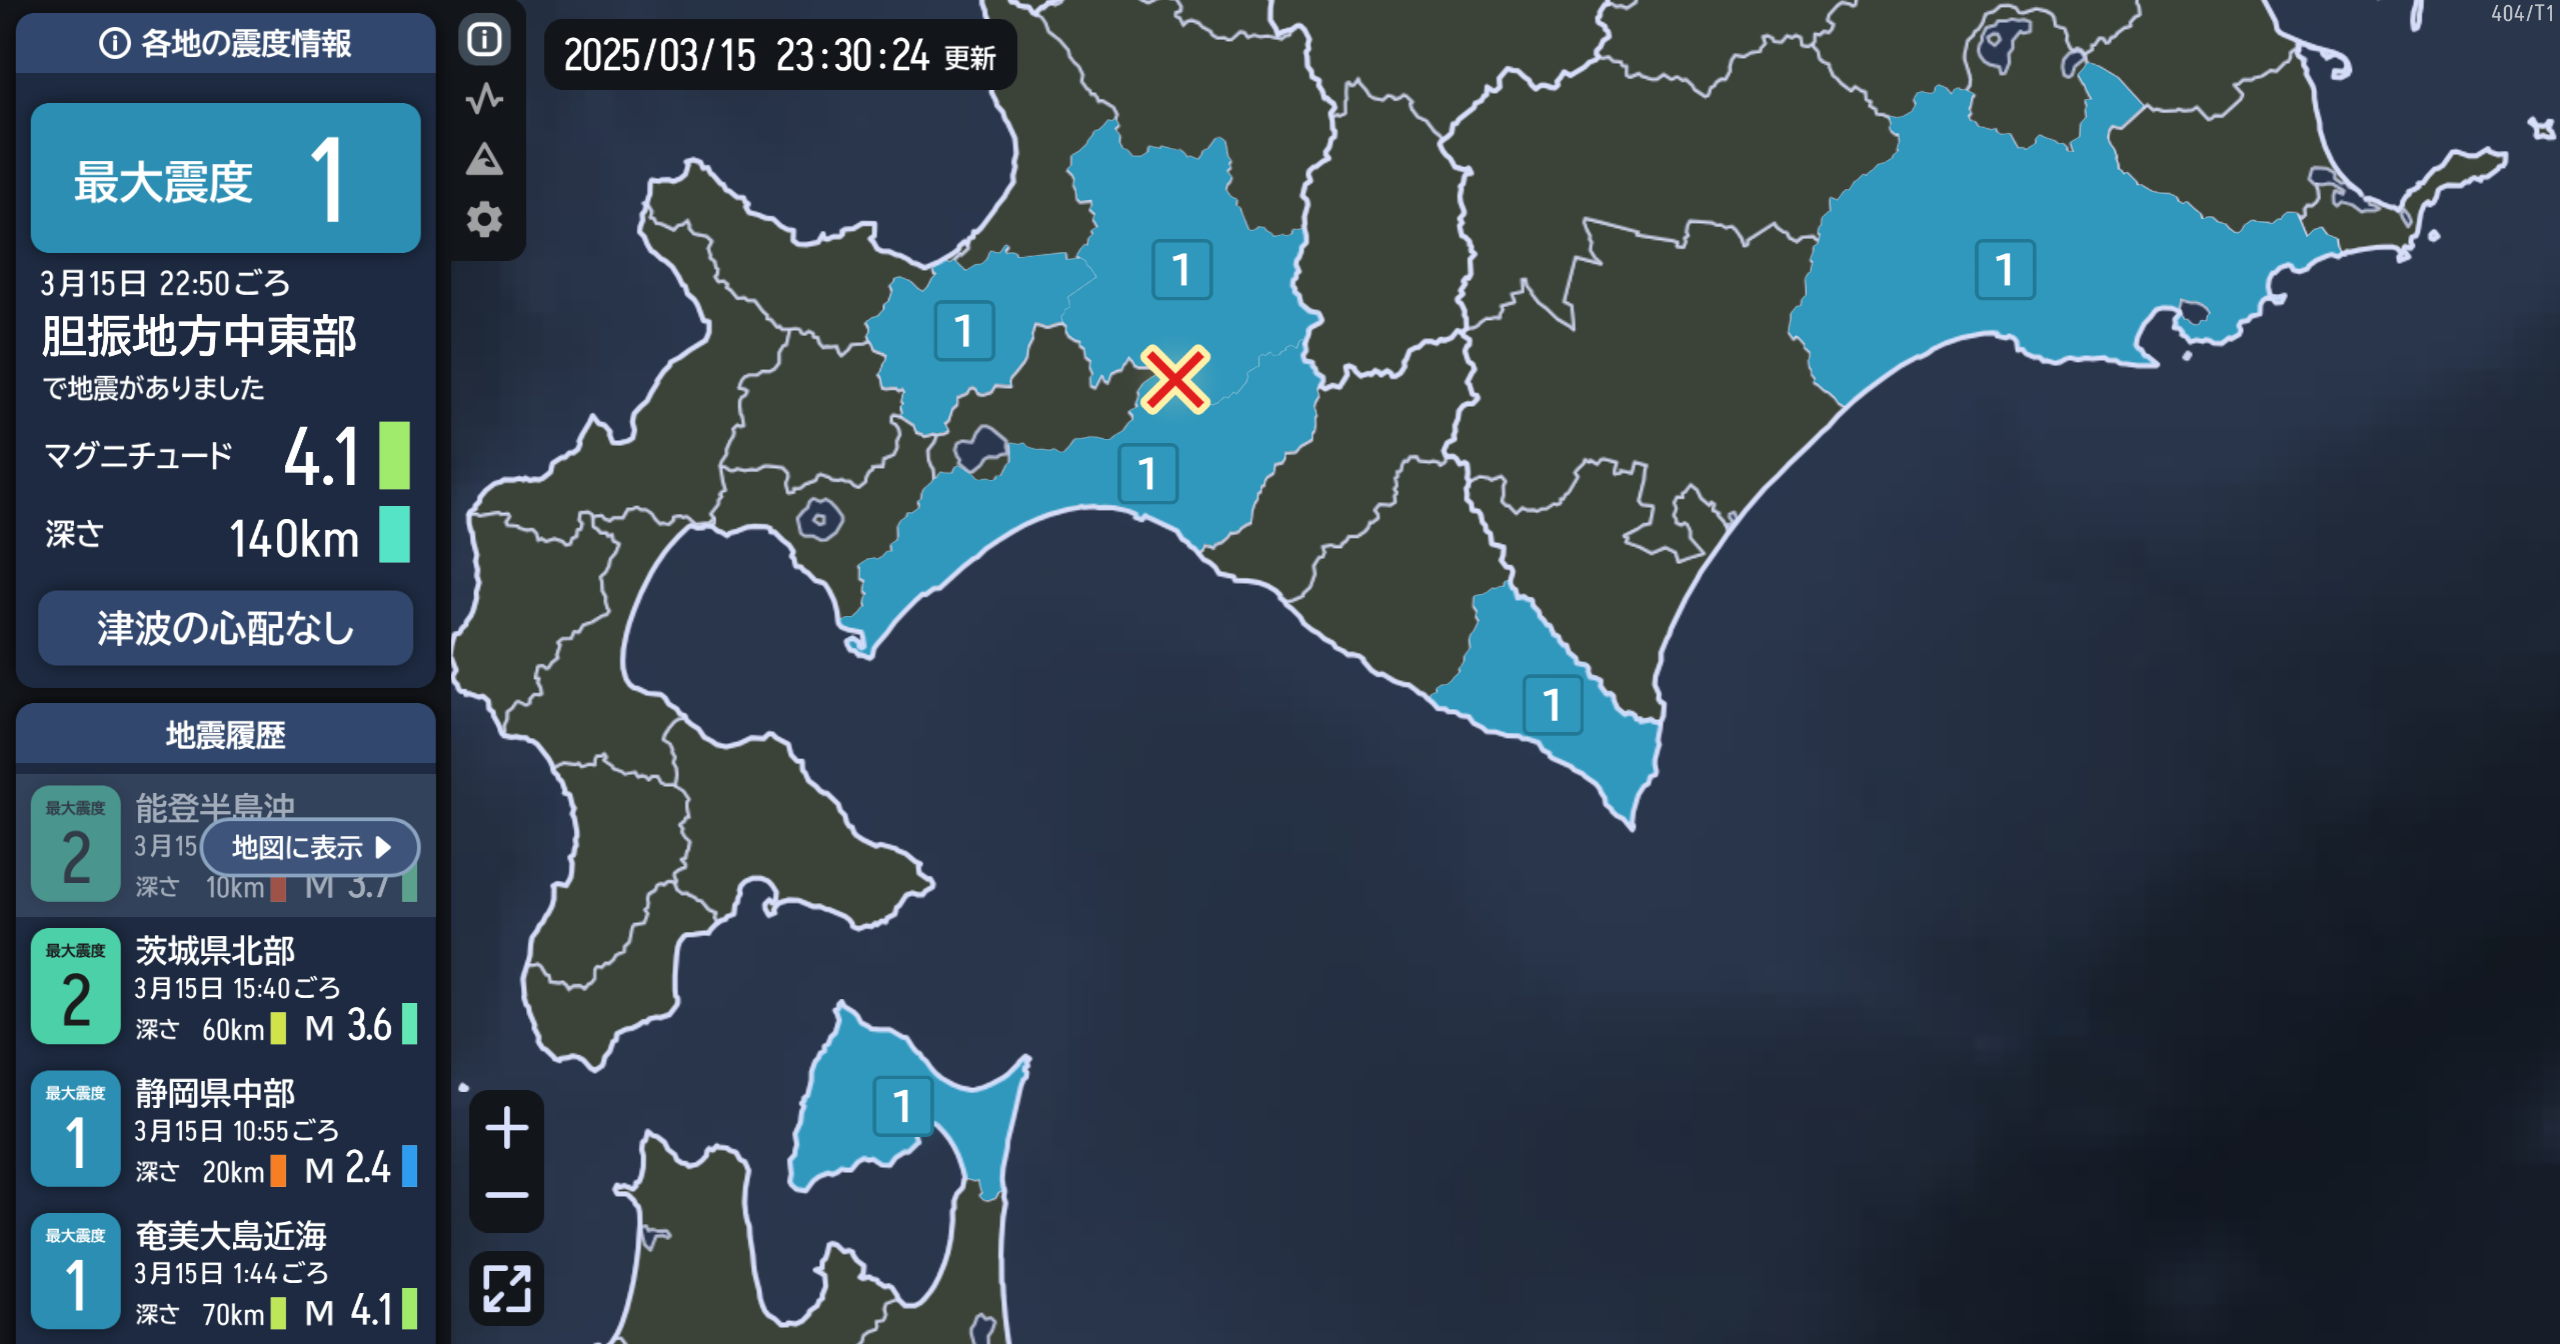
\includegraphics[width=0.7\linewidth]{srev-past-page.png}
    \caption[Past earthquake pages for KEVI and SREV]{Past earthquake pages\\
        Top: KEVI; Bottom: SREV}
    \label{fig:kevi-srev-past-page}
\end{figure}
\begin{figure}[htp]
    \centering

    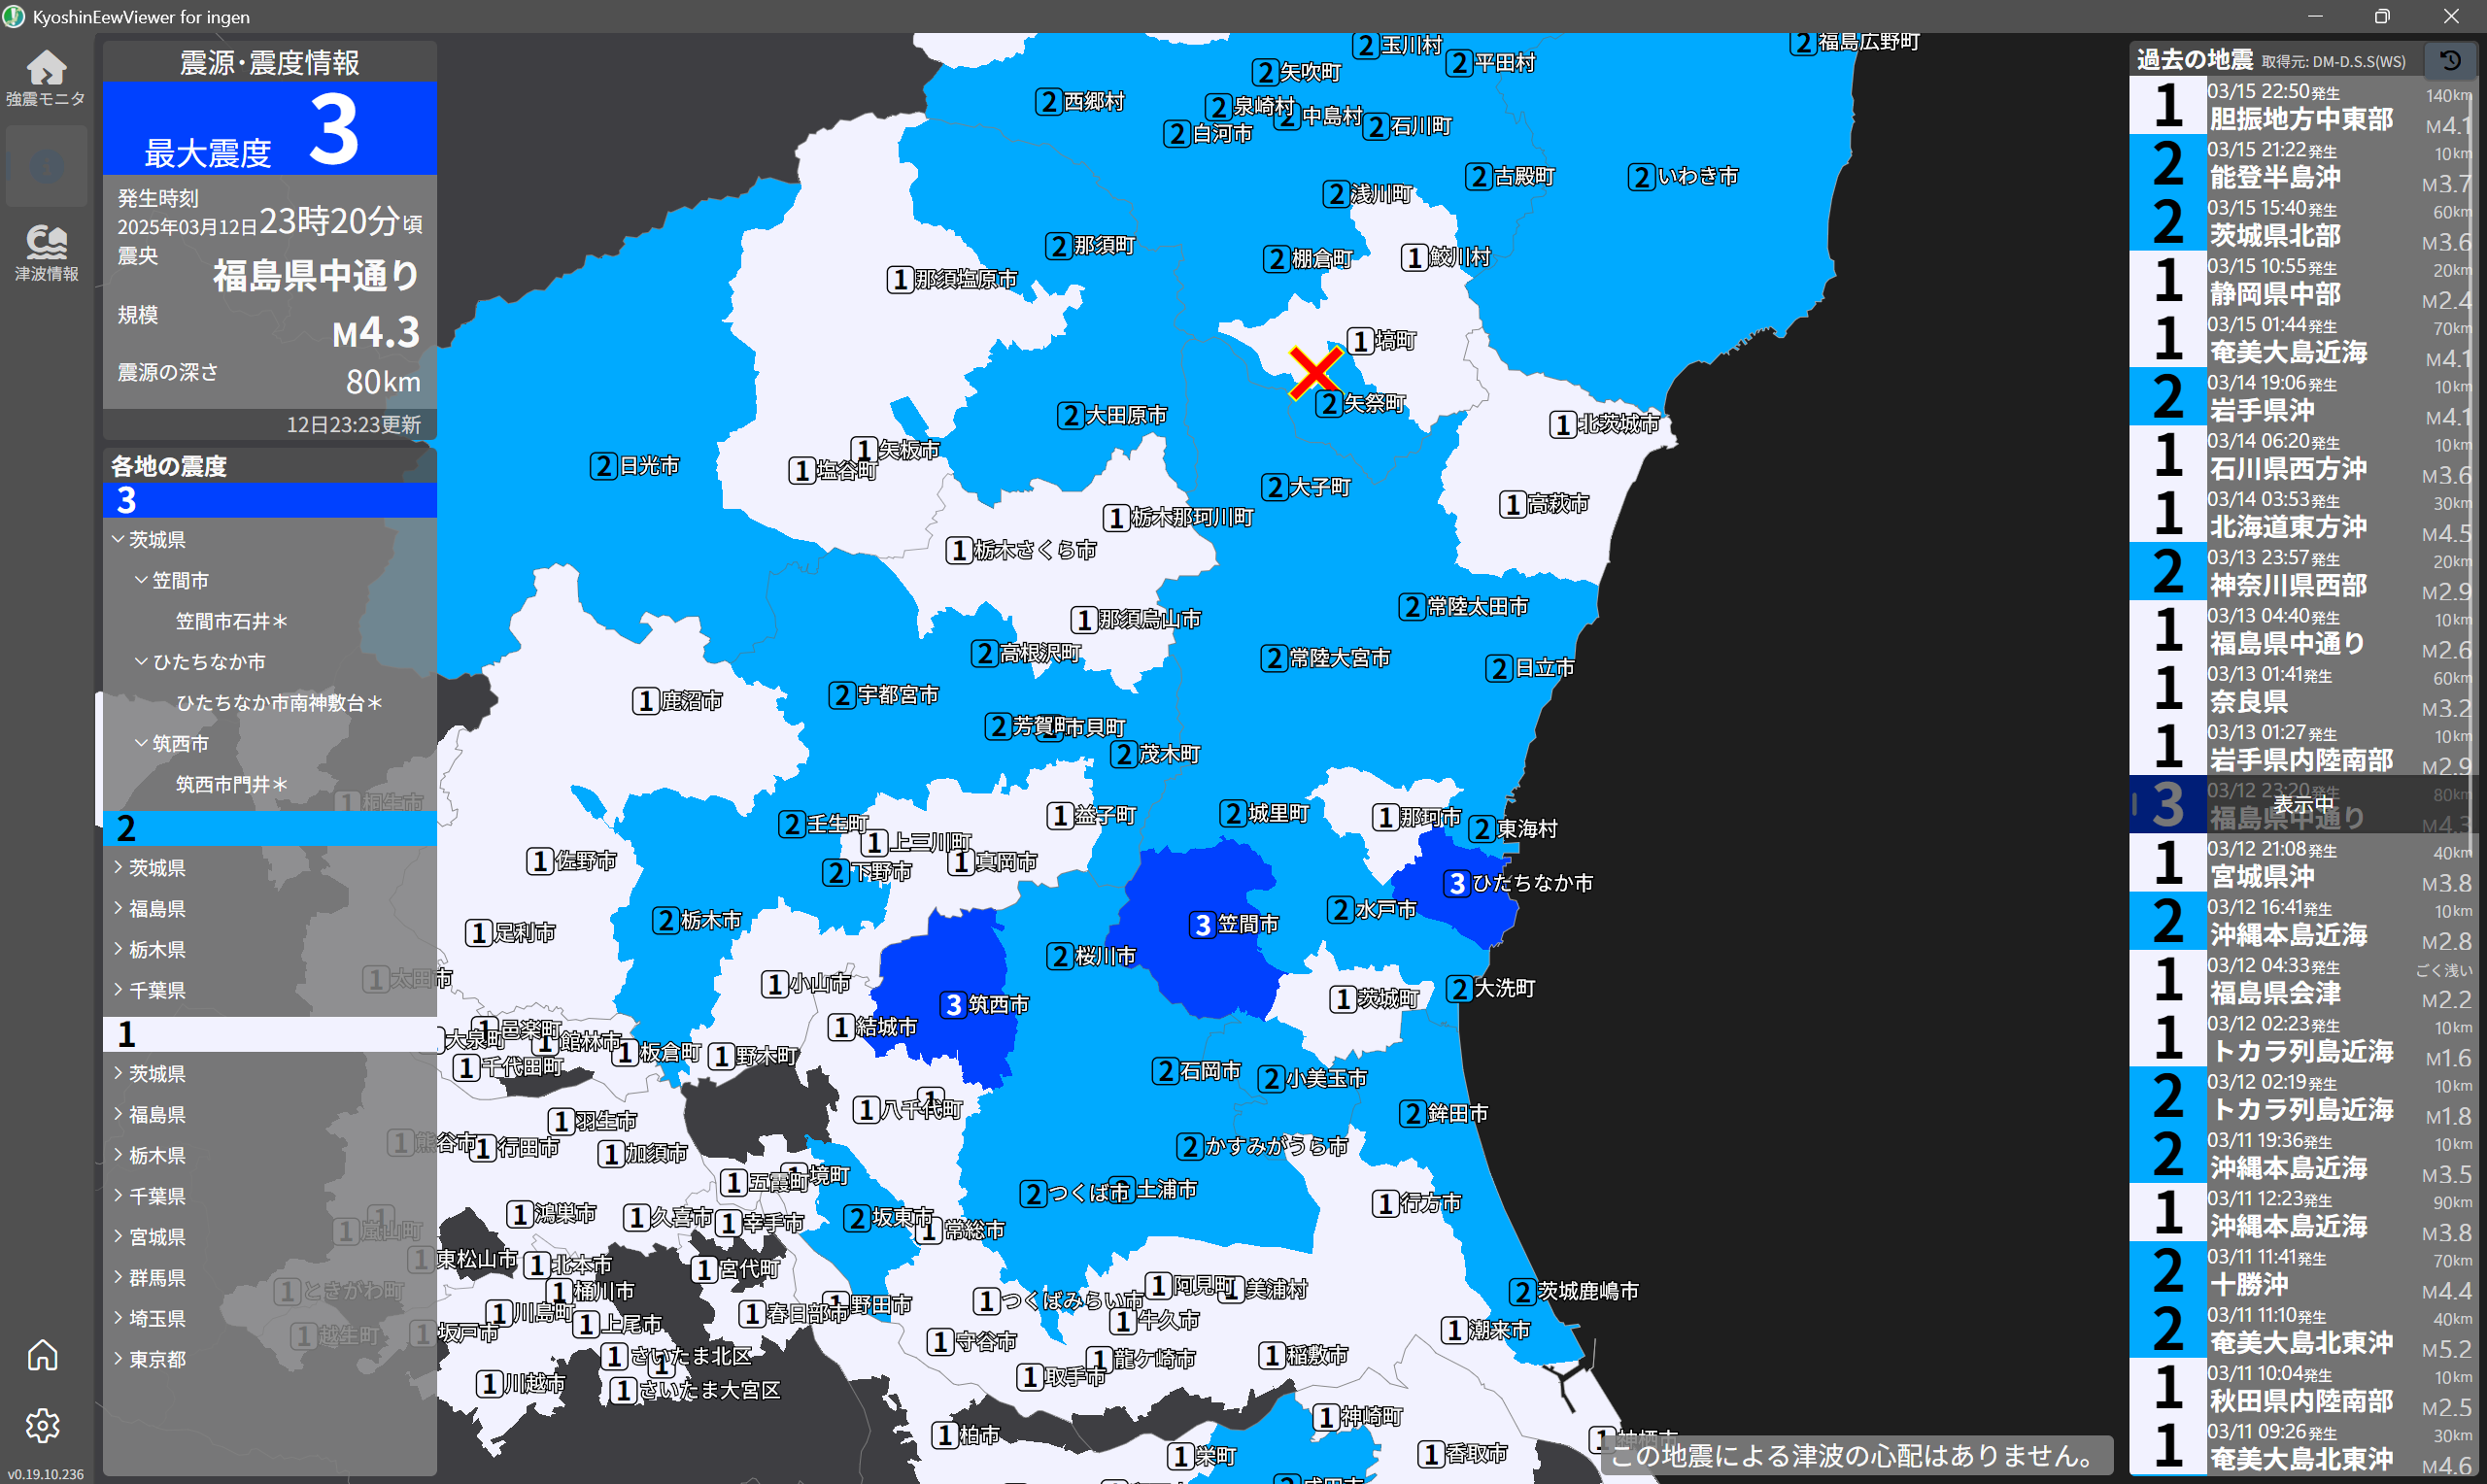
\includegraphics[width=0.8\linewidth]{kevi-map.png}
    \caption{Display of observation stations and regions of KEVI}
    \label{fig:kevi-map}
\end{figure}

In particular for KEVI, there is also a tree structure on a panel displaying the details of the observed intensities by hierarchy structure, consisting of prefectures, skipping regions, then districts, then the exact observation stations, as shown in \autoref{fig:kevi-intensity-tree}.

\begin{figure}[htp]
    \centering

    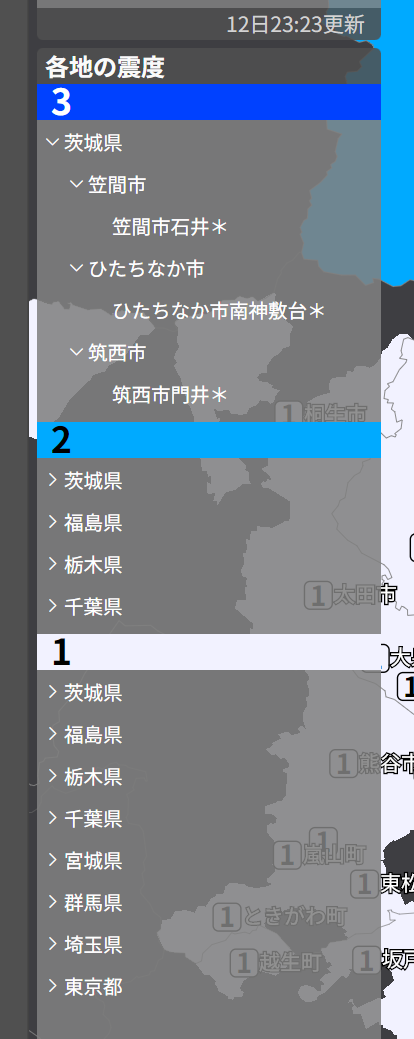
\includegraphics[width=0.4\linewidth]{kevi-intensity-tree.png}
    \caption{Intensity tree on side panel of KEVI}
    \label{fig:kevi-intensity-tree}
\end{figure}

As for SREV, the selected earthquake will be displayed on the map and coloured by region, but no information on observation stations will be provided. For JQuake, it is impossible to select a particular earthquake, but only possible to replay the past earthquake, and jump to an external weather service to view the details, as shown in \autoref{fig:jquake-sidebar-options}.

\begin{figure}[htp]
    \centering

    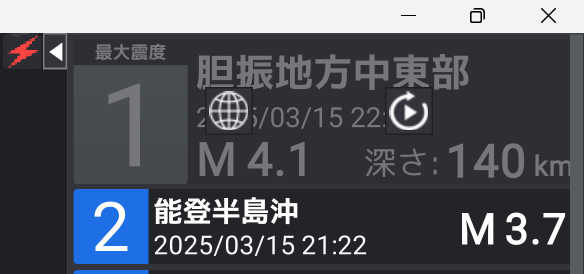
\includegraphics[width=0.3\linewidth]{jquake-sidebar-options.png}
    \caption[Sidebar options of JQuake]{Sidebar options of JQuake\\
        Globe: Link to Yahoo! weather service page for earthquake;\\
        Time-lapse: Replay of earthquake}
    \label{fig:jquake-sidebar-options}
\end{figure}

A significant difference between the applications is how they split the different functionalities. For KEVI and SREV, there are separate pages for real-time monitoring, past-earthquake viewing and tsunami warnings, as shown in \autoref{fig:kevi-real-time-tsunami} for KEVI, and \autoref{fig:srev-real-time-tsunami} for SREV.

\begin{figure}[htp]
    \centering

    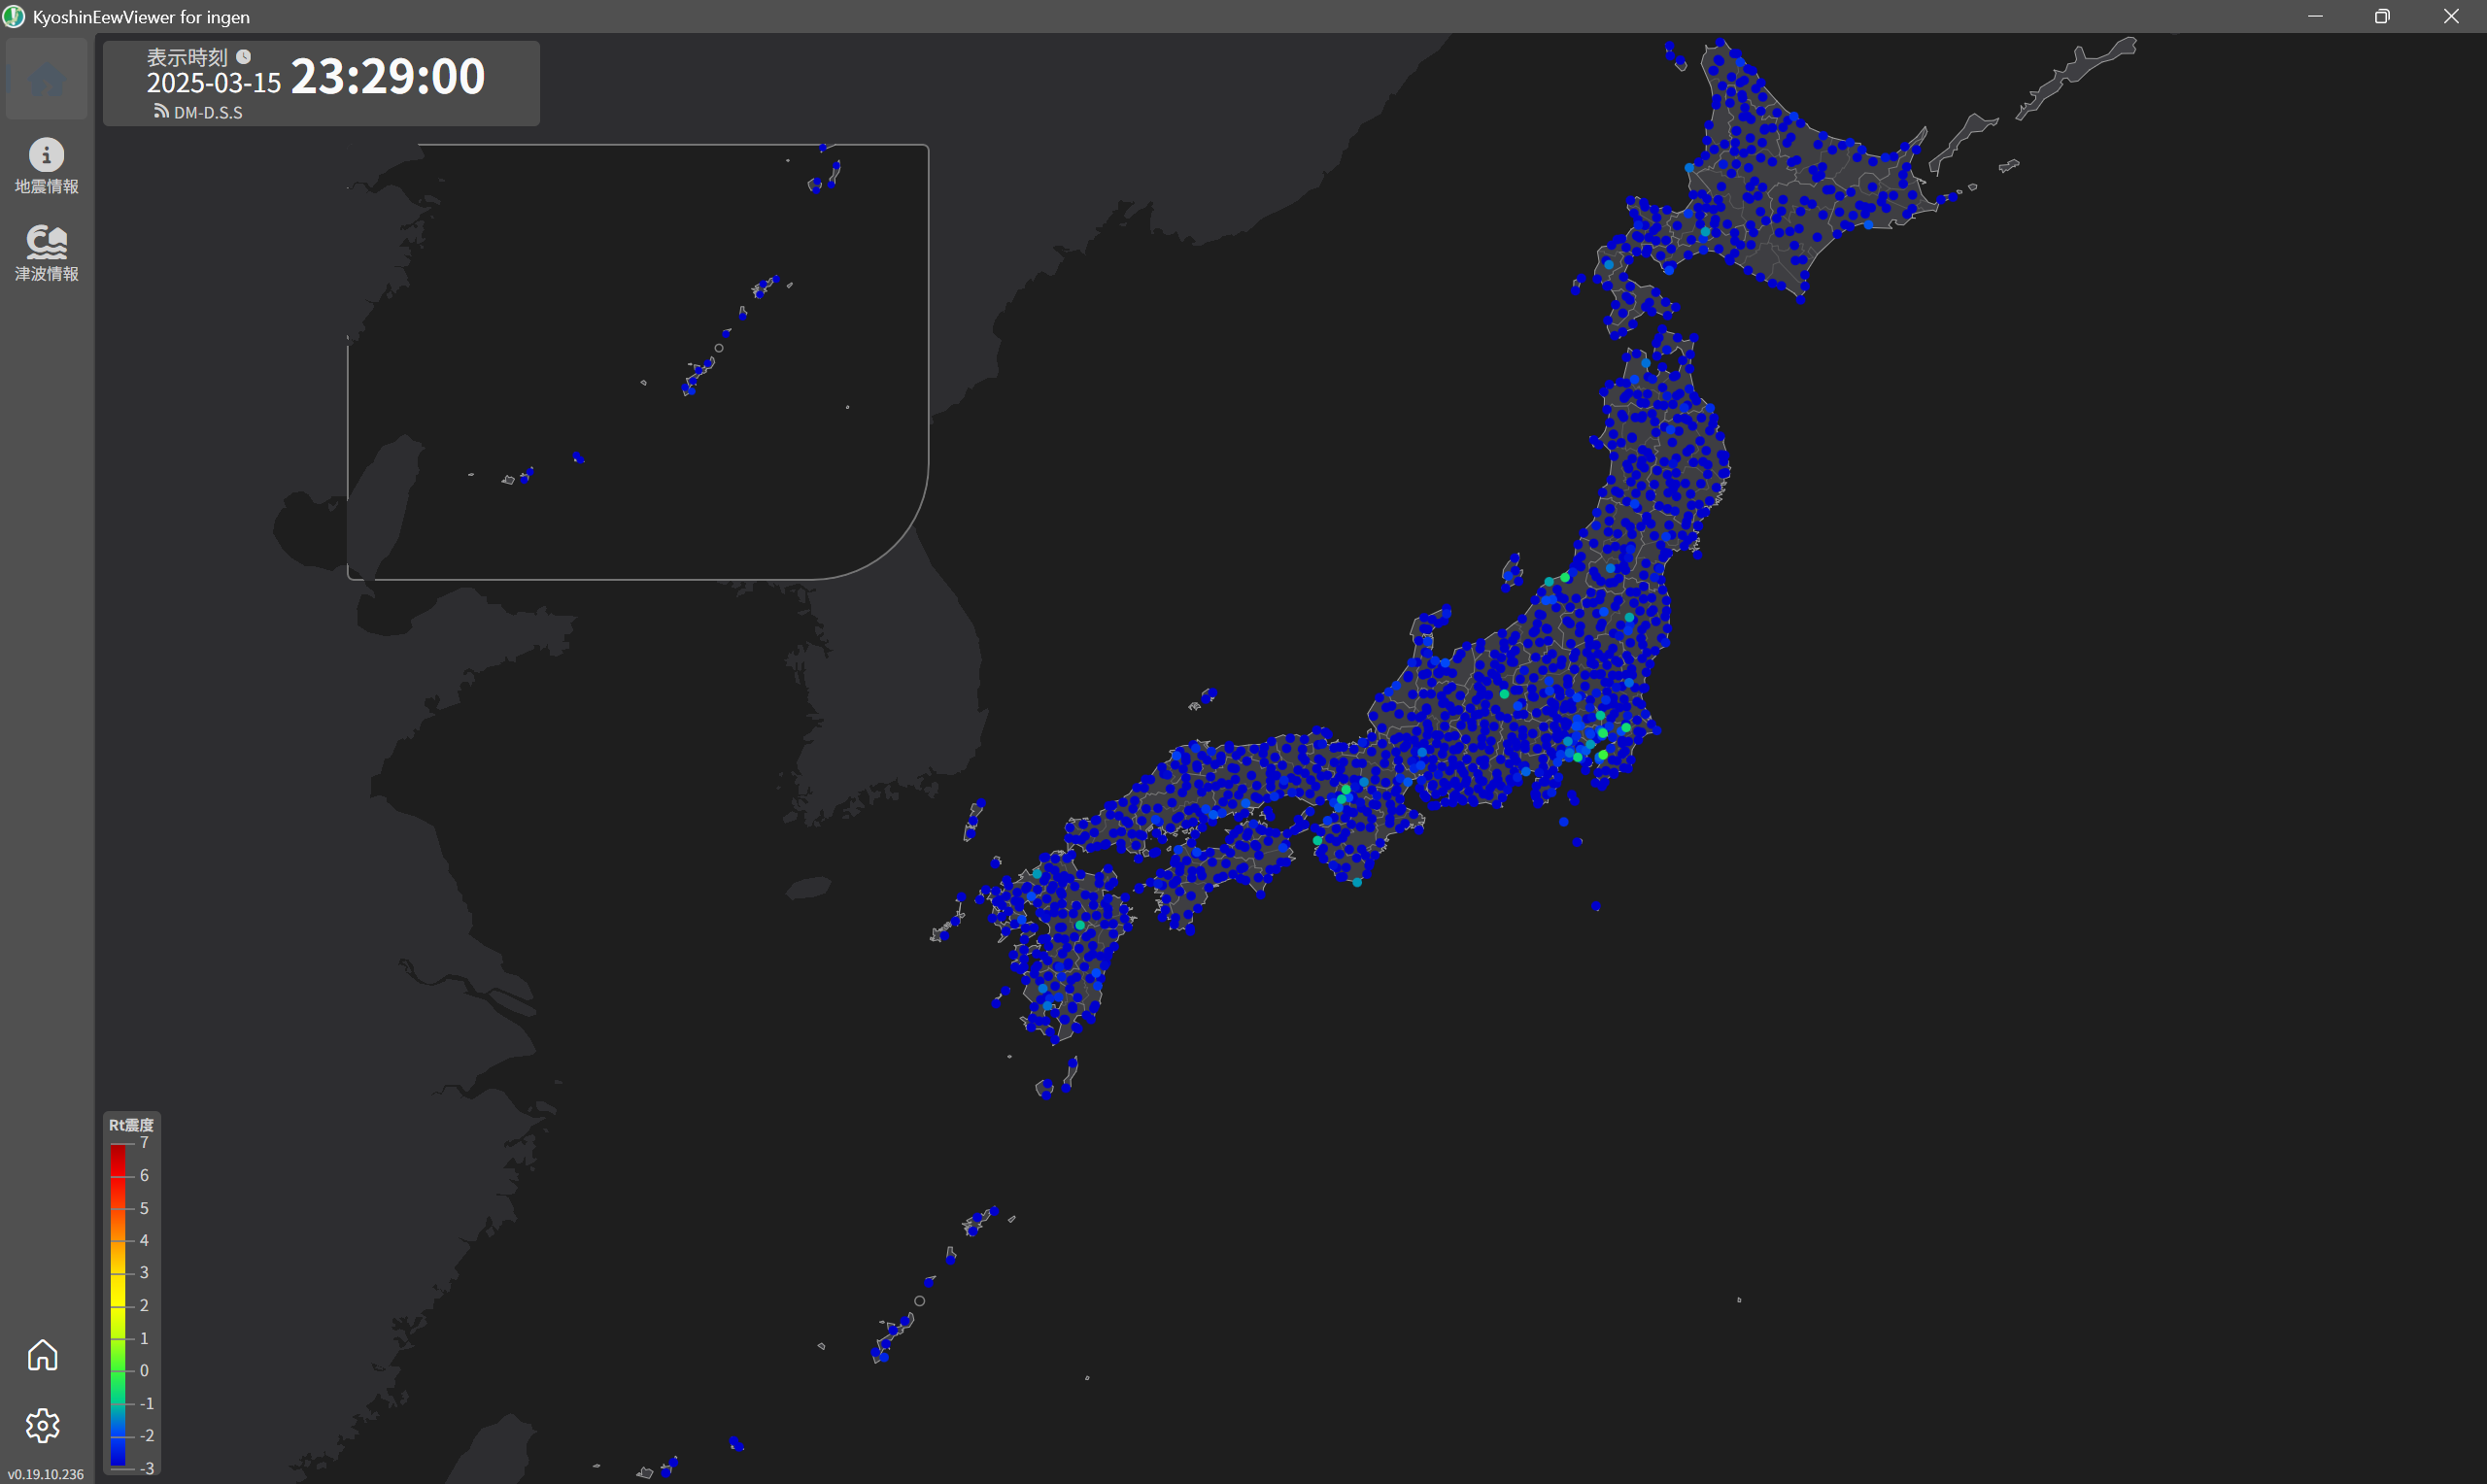
\includegraphics[width=0.7\linewidth]{kevi-real-time-page.png}
    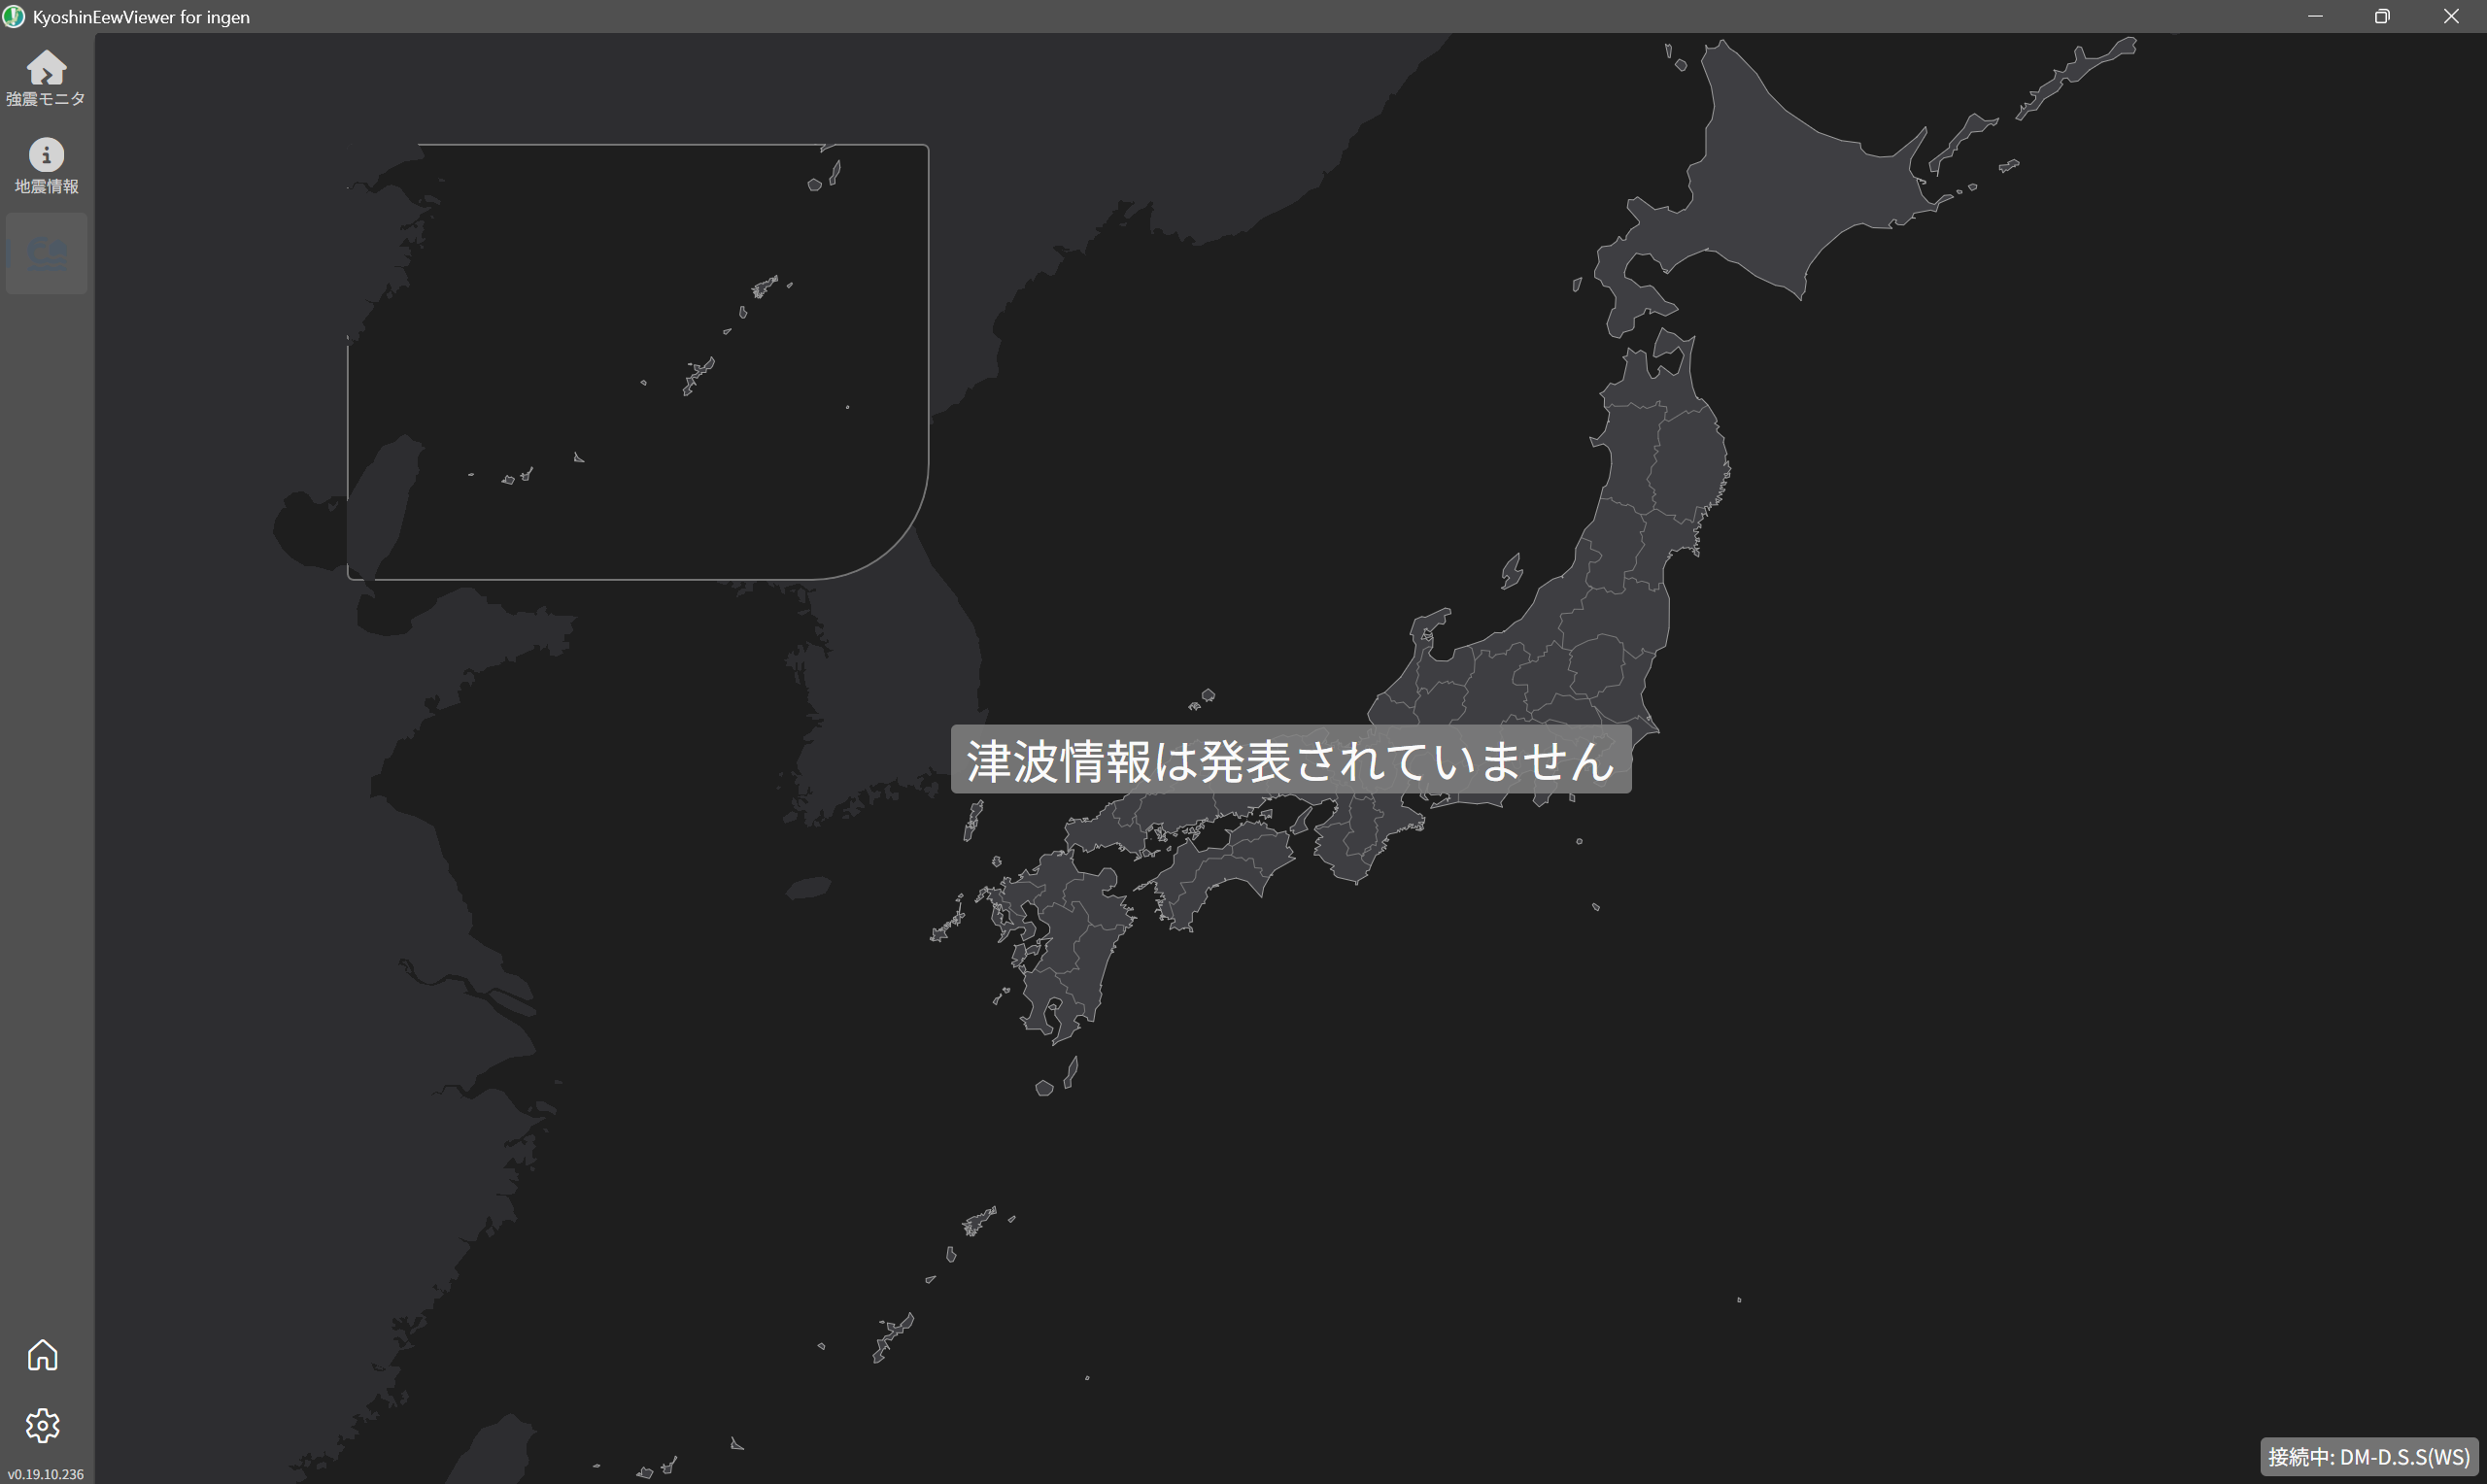
\includegraphics[width=0.7\linewidth]{kevi-tsunami.png}
    \caption{Real-time and tsunami pages of KEVI}
    \label{fig:kevi-real-time-tsunami}
\end{figure}

\begin{figure}[htp]
    \centering

    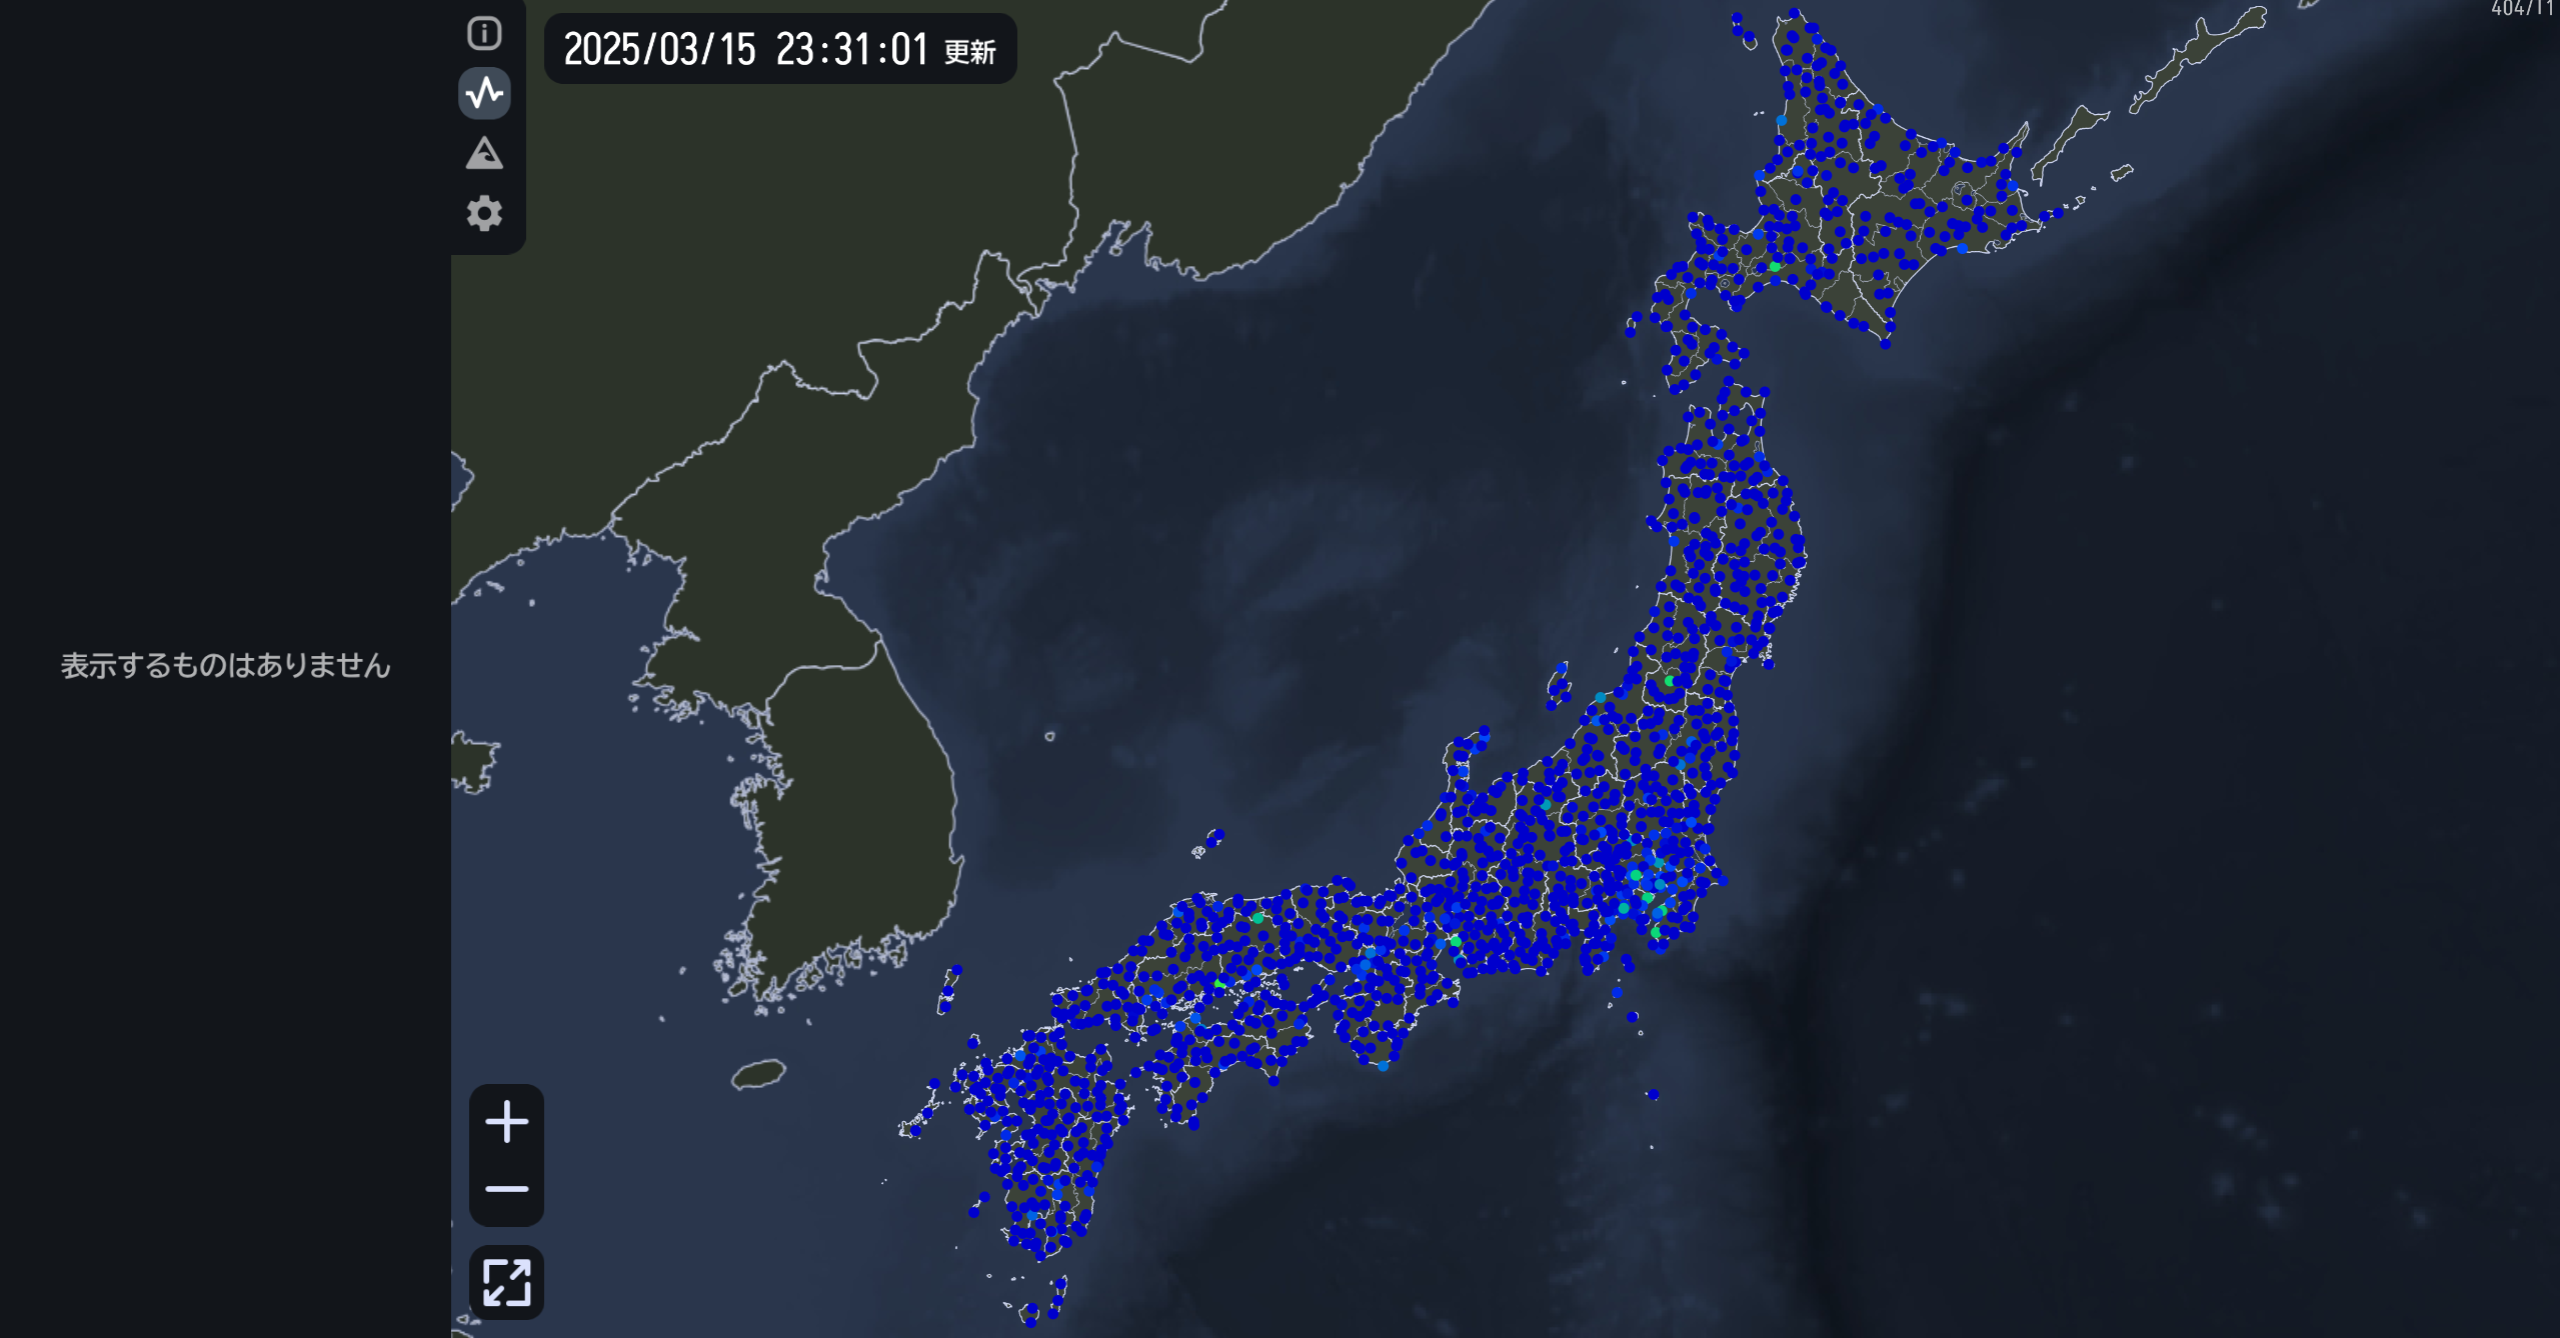
\includegraphics[width=0.7\linewidth]{srev-real-time-page.png}
    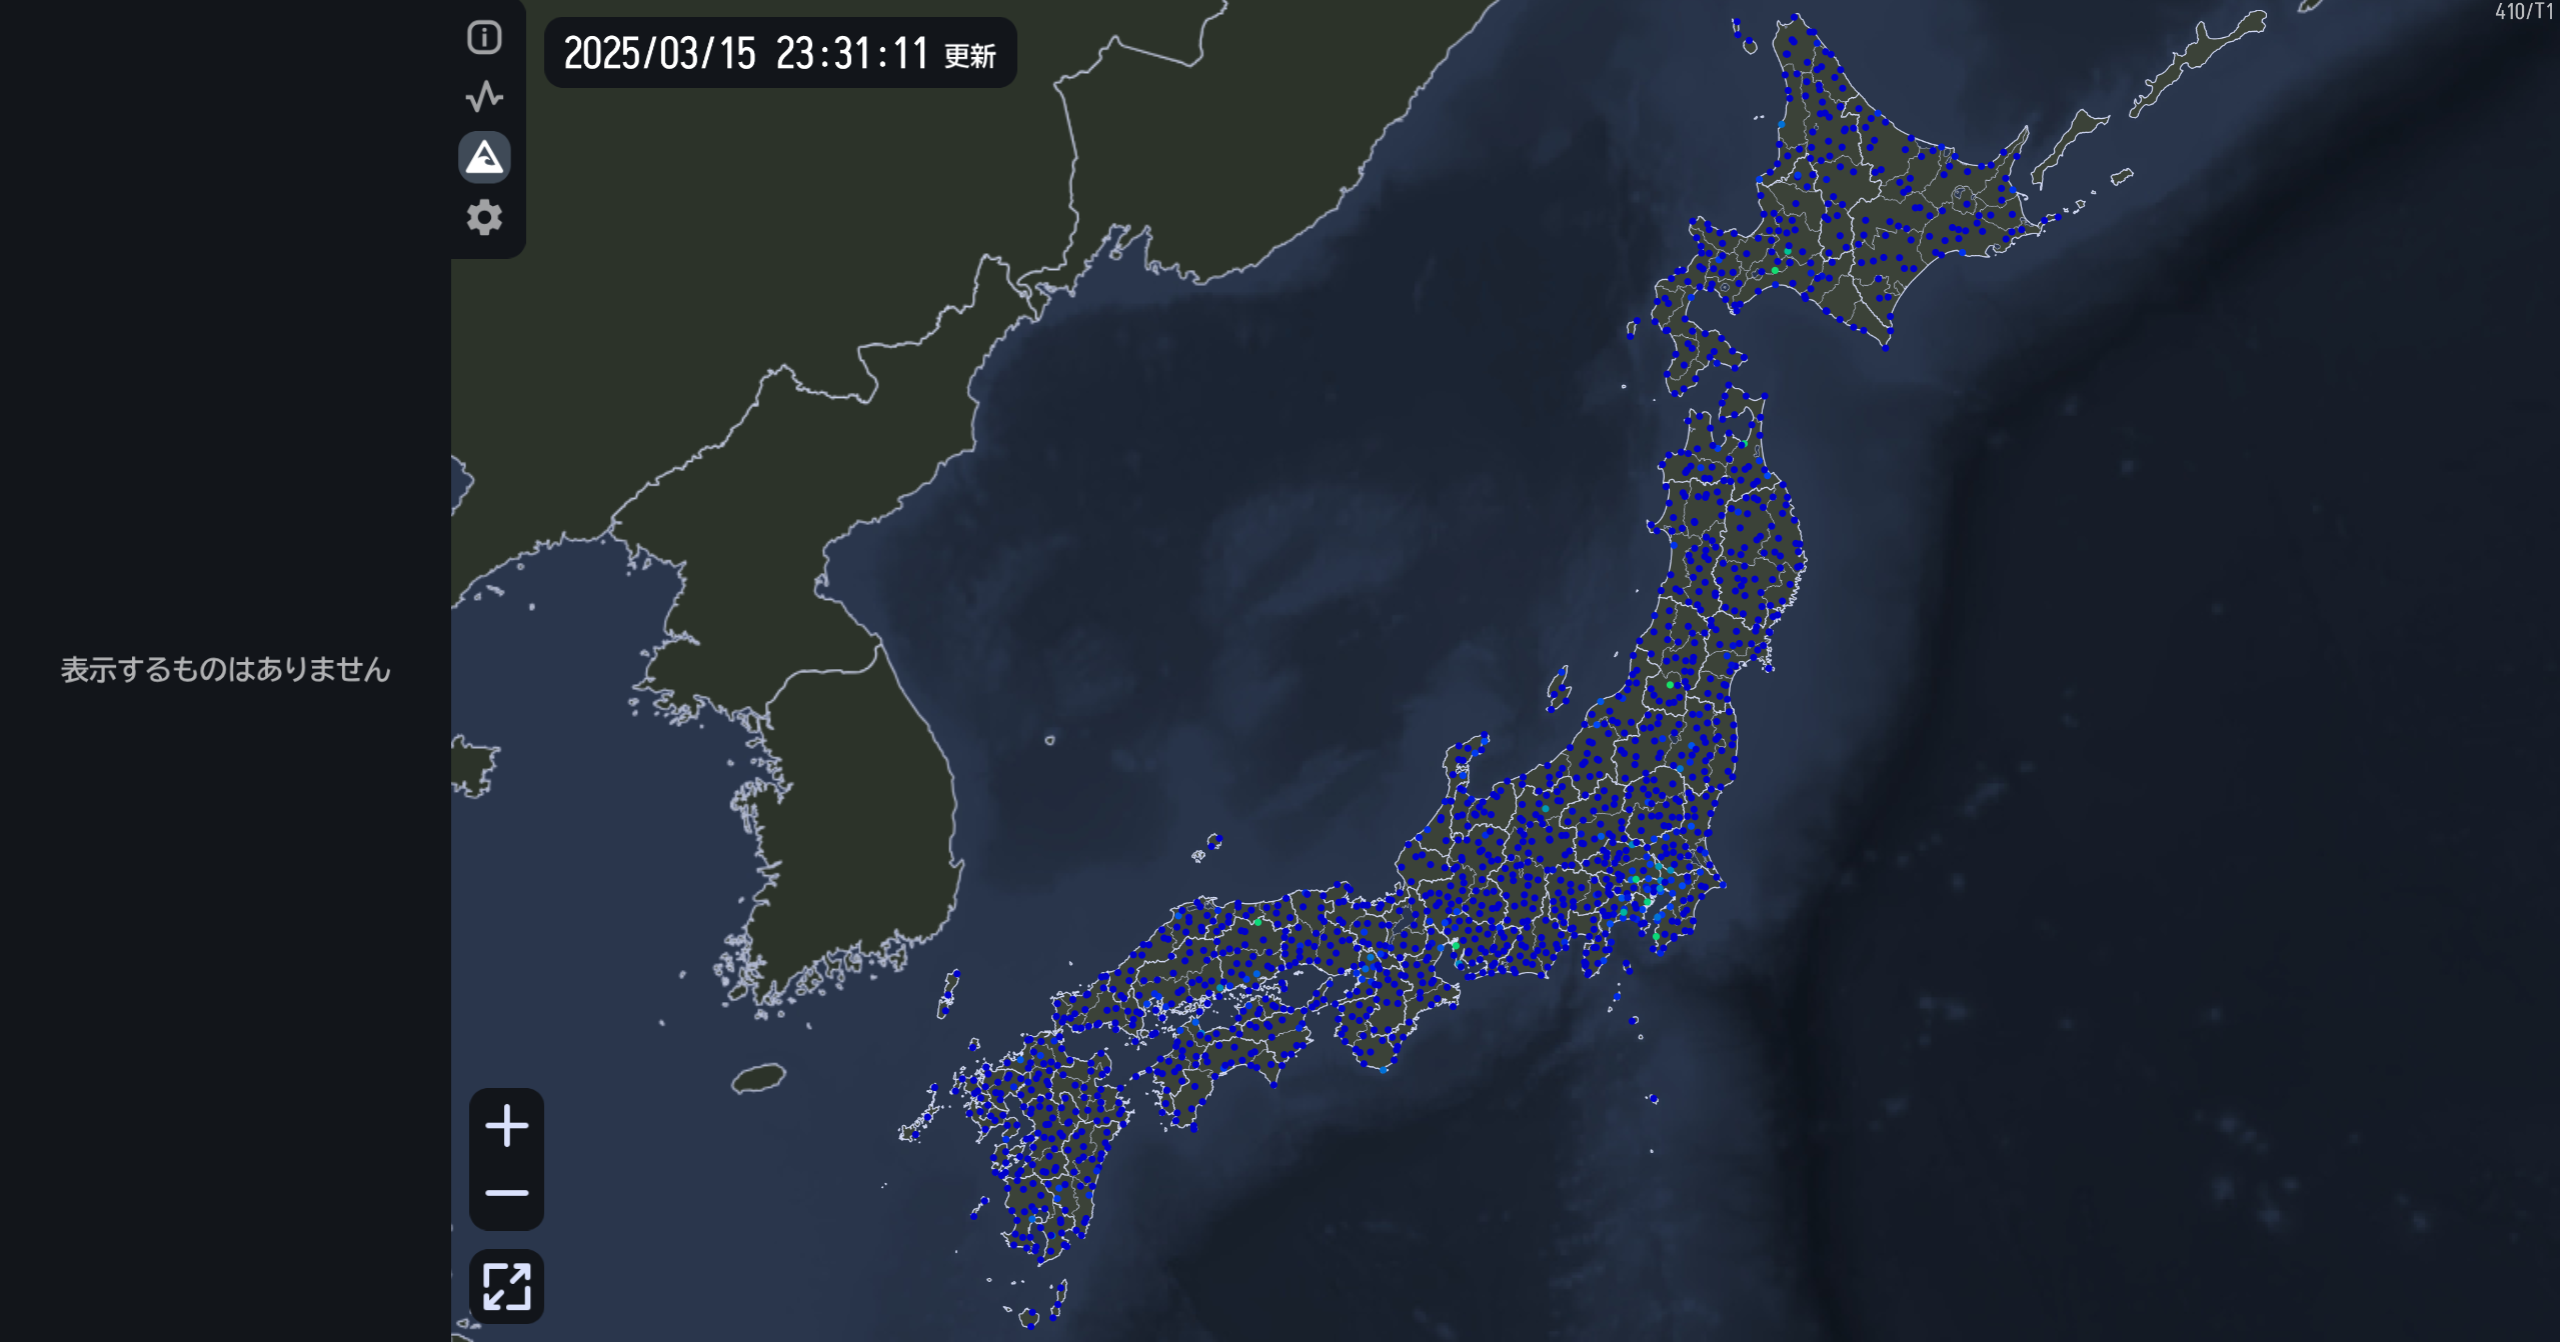
\includegraphics[width=0.7\linewidth]{srev-tsunami-page.png}
    \caption{Real-time and tsunami pages of SREV}
    \label{fig:srev-real-time-tsunami}
\end{figure}

On the contrary, since JQuake's map only supports replay and real-time functionality (EEW and tsunami), there is only one page, as shown in \autoref{fig:jquake-main-page}. Quarog will automatically switch the map to display EEWs if EEWs are issued, and change the sidebar to display the predicted intensities of EEWs, as shown in \autoref{fig:quarog-monitor-features}.

\begin{figure}[htp]
    \centering

    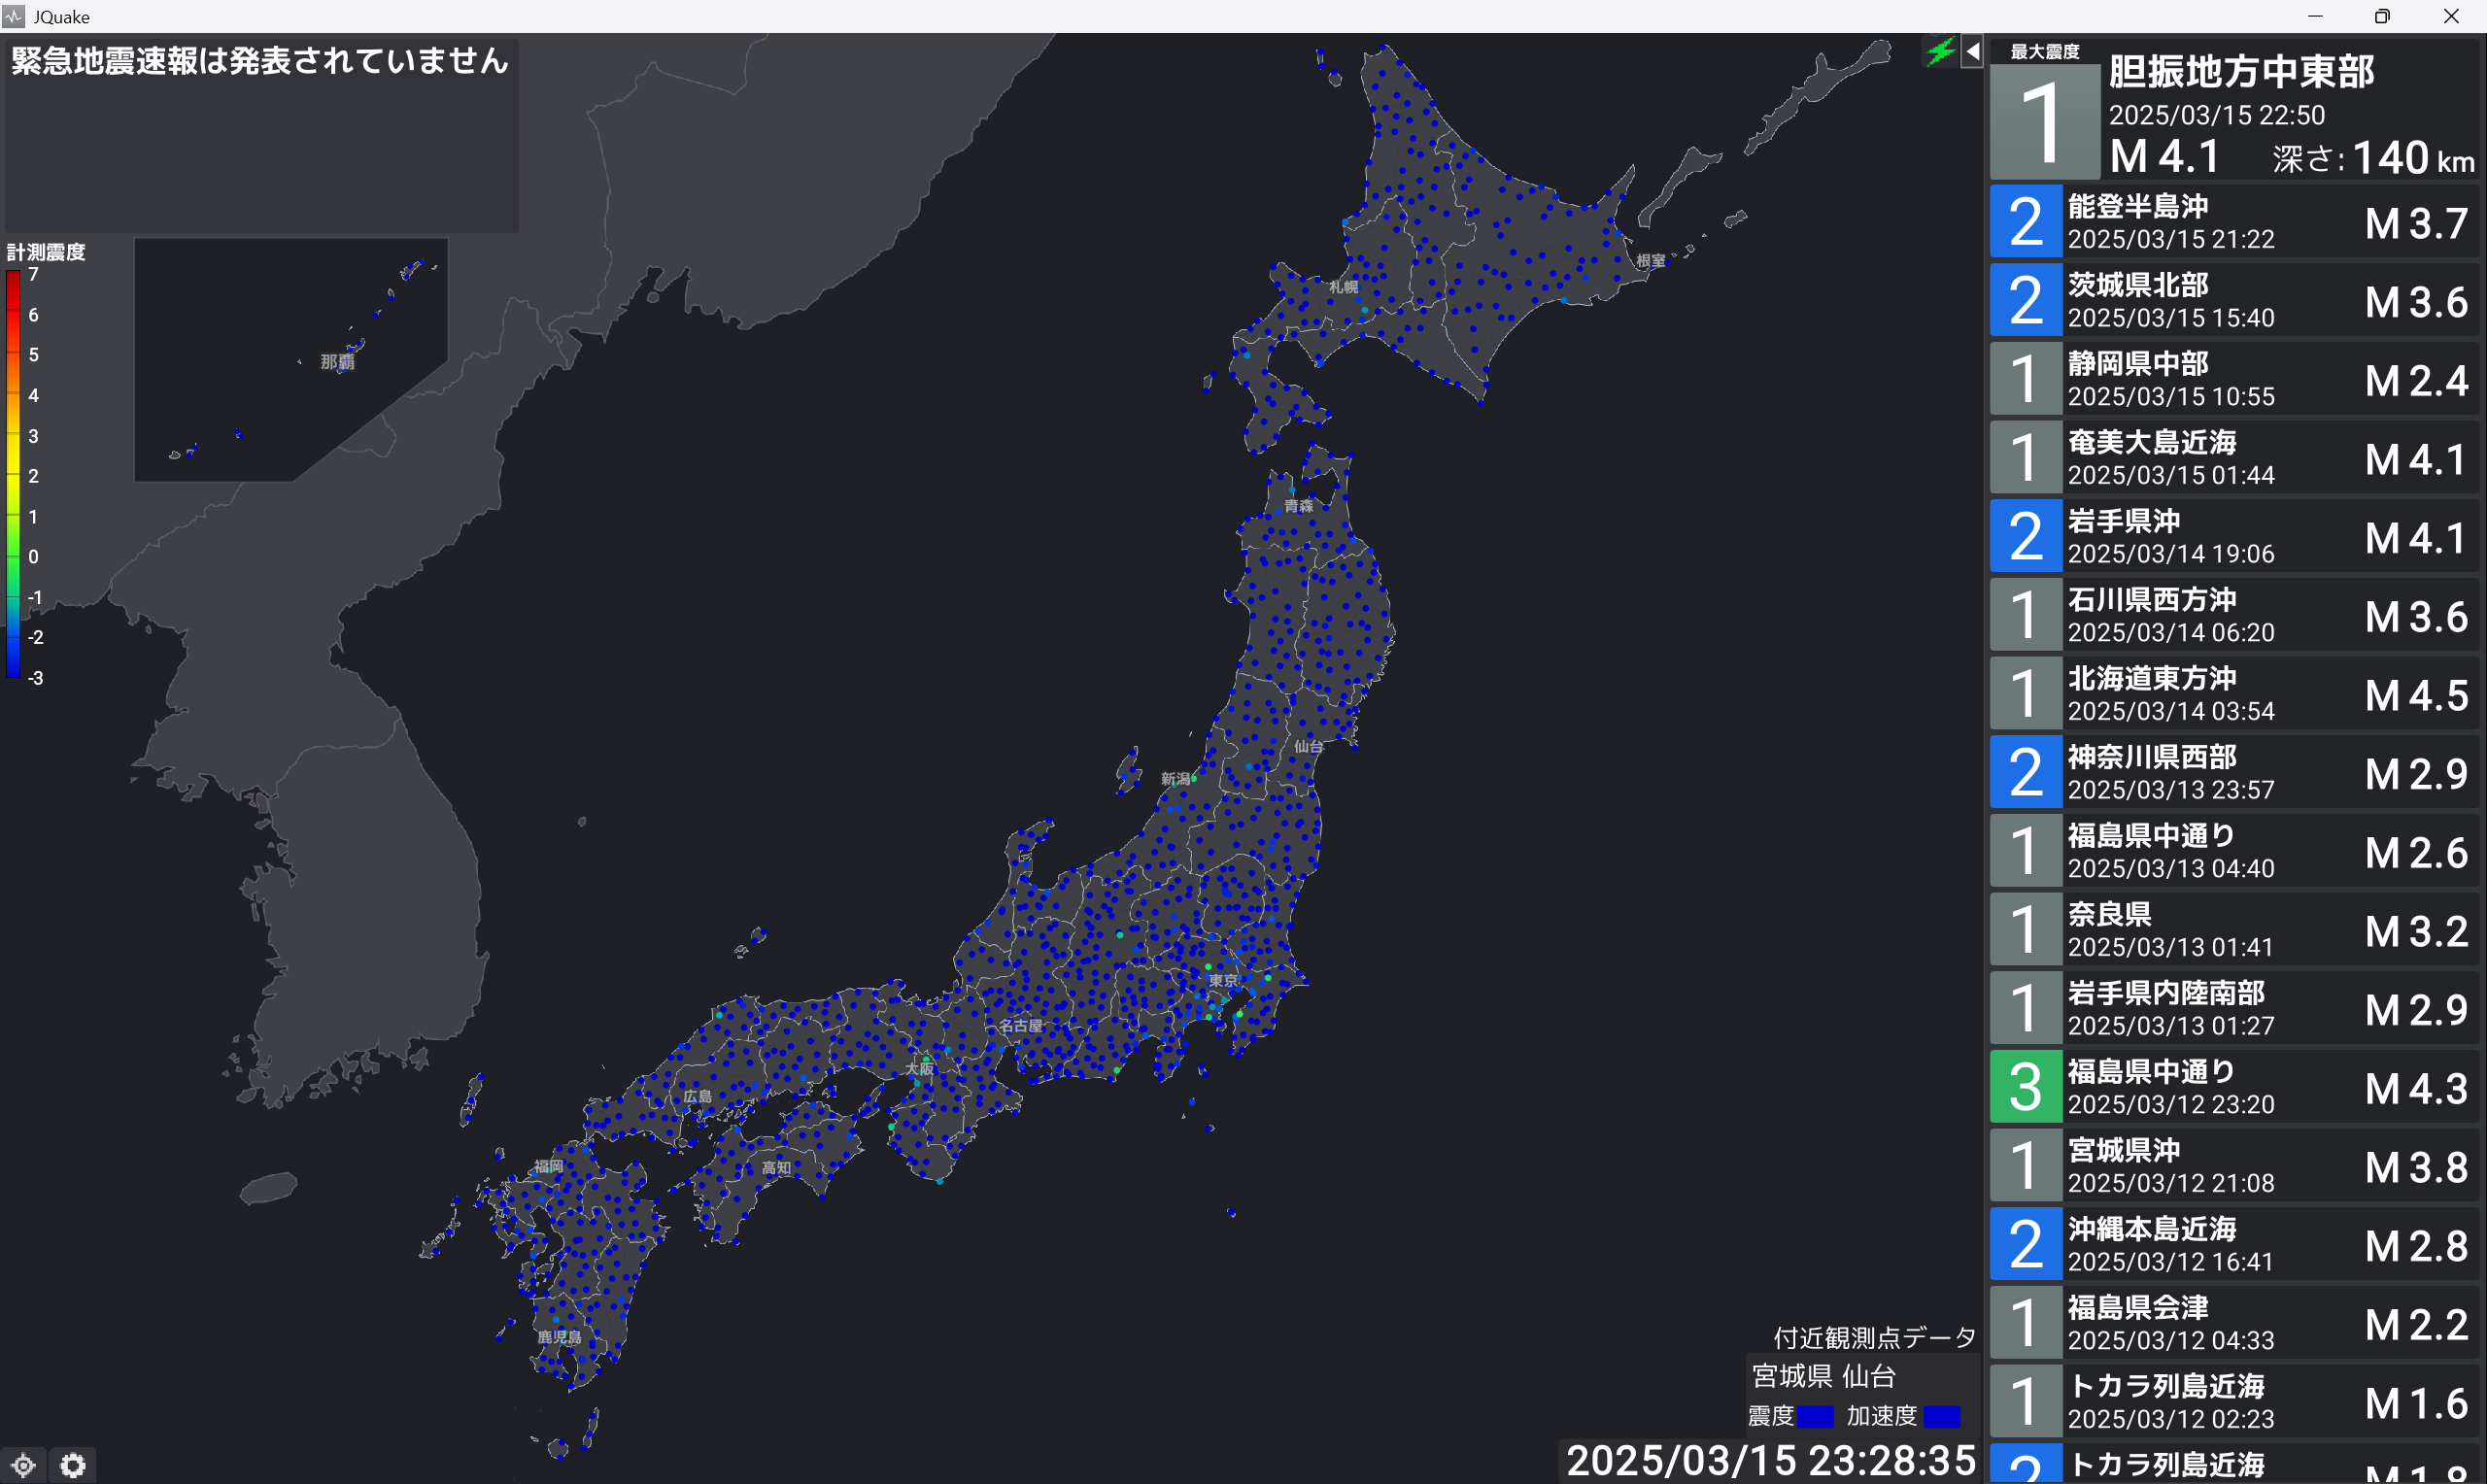
\includegraphics[width=0.6\linewidth]{jquake-main-page.png}
    \caption{Main page for JQuake}
    \label{fig:jquake-main-page}
\end{figure}

\section{Features of proposed solution}

Based on the potential user/client interview results, and the research into the existing solutions, the following key features should appear in the solution, since they are essential to earthquake monitoring applications:
\begin{enumerate}
    \item DM-D.S.S. Login functionality (for the data source)
    \item Real-Time Sensor Shake Intensity Data
    \item EEW Visualisation (w/ Calculated Seismic Wavefronts)
    \item Past Earthquake List (w/ Option to review details)
    \item Tsunami Warning Visualisation
\end{enumerate}

However, due to the limitation of time, the following functionalities are excluded from the scope of this project, which include mostly the customisation parts, ranked in decreasing importance:
\begin{enumerate}
    \item Shake detection algorithm (based on real-time sensor data)
    \item User-Defined Key Monitor Point
    \item (Customisable) Sound Alert
    \item Customisable Colour Theme
\end{enumerate}

The following features are considered too complicated for the scope for this project and the time constraints, hence not considered:
\begin{enumerate}
    \item Replay (due to a server needing to store past data)
    \item Sub-Map for the Okinawa Area (due to the difficulty in implementation)
\end{enumerate}

With those key features implemented, the application should mirror all essential functionalities of an earthquake monitoring application, as compared to the four existing solutions above.

\section{Critical Path}

The functionality of this application can essentially be divided into \(1+2+1+a+b\) steps, where the 1 is to receive information from the API/WebSocket provided by DM-D.S.S. and NIED, and 2 is to, briefly saying:
\begin{enumerate}
    \item Real-time Monitoring: Produce a real-time map to monitor real time vibration and plot real-time EEW/tsunami warnings
    \item Past-earthquake Viewing: Produce a menu to select an earthquake to display information on the map.
\end{enumerate}

The next 1 is to merge these two functions, specifically the functionality to switch back to the real-time monitoring option immediately when a new EEW is released (to make sure the user does not miss any information on real-time EEWs while looking at past earthquake information).

The \(a\) is to implement a setting page for customisation and some additional features, and the \(b\) is to implement additional functionalities that are excluded from this project, but could be completed if there is time.

\subsection{Part 1. NIED and DM-D.S.S. API/WebSocket Connection}
\begin{enumerate}
    \item Investigate into the list of APIs/WebSockets that should be used by the application.
    \item Investigate into patterns of the response data, and design the classes/DTOs using correct OOP patterns such as inheritance and composition.
    \item Implement classes/DTOs to convert the information into C\# objects.
    \item Implement classes/DTOs to convert telegrams into C\# objects.
    \item Use API Key to test the functionality of this system.
    \item Implement OAuth 2 login functionality to reduce complexity and increase security.
\end{enumerate}

\subsection{Part 2a. Real-time Monitoring Map}
\begin{enumerate}
    \item Display a map in the application.
    \item Extract the data from the real-time measured intensities of observation stations from the data source.
    \item Display the data on the map using a default colour scheme at the correct positions.
    \item Colour the monitoring points using a colour scheme on the map.
    \item Investigate into and implement an algorithm to calculate seismic wave fronts, using necessary data provided by the JMA.
    \item Plot and colour real time EEWs, considering special cases such as:
          \begin{itemize}
              \item Cancellation of EEW;
              \item Upgrade from EEW Forecast to EEW Warning;
              \item Multiple Earthquakes (hence displaying multiple epicentres, and switching between earthquakes in details display);
              \item Assumed Hypocentre (hence using a different hypocentre symbol to display).
          \end{itemize}
    \item Colour areas on the map with the maximum expected intensity.
    \item Plot on the map the hypocentre of the earthquake, using the correct symbol.
    \item Plot and colour real time tsunami warnings.
\end{enumerate}

\subsection{Part 2b. Past-earthquake Viewing}
\begin{enumerate}
    \item Plot a sidebar of a list to display path earthquakes.
    \item Provide a button to refresh the sidebar, and another one to load more earthquakes.
    \item Provide a functionality to choose an earthquake from the sidebar to view the detailed information on the earthquake (e.g. magnitude, epicentre, time, additional message).
    \item Plot the hypocentre of the earthquake.
    \item Plot the observed maximum intensities on the map by regions.
    \item Plot the intensities measured by each observation station on the map.
    \item Provide external link to view earthquake in the weather service provider website.
\end{enumerate}

\subsection{Part 3. Joint functionality}
\begin{enumerate}
    \item Provide sidebar to switch between real-time monitoring and past-earthquake viewing, and settings options.
    \item Implement automatic functionality to switch back to real-time earthquake when an EEW/Tsunami Warning is being published.
\end{enumerate}

\subsection{Part 4. Setting page for customisation}
\begin{enumerate}
    \item Provide a text box to input the API Key, and a button to confirm the API Key.
    \item Provide a button to connect and authorise with OAuth 2.0.
    \item Provide a button to connect to the WebSocket.
    \item Display a list of current WebSocket connections, and provide a button to refresh such list.
    \item Provide two dropdown menus, to choose the sensors to display on the real-time map (all sensors, or borehole only), and the data to display (real time intensity, PGA, PGV, PGD, etc.).
\end{enumerate}

\subsection{Part 5. Additional functionalities}
\begin{enumerate}
    \item Investigate into and implement an algorithm to detect shakes based on the observed data.
    \item Provide functionality to define a specific point on the map, and display the measured intensity at that point.
    \item Play sound alerts when EEW/Tsunami warnings are received.
    \item Provide custom sound alert settings to specify the file to the sound alert.
    \item Provide custom colour theme settings to specify the colour scheme of the colouring on the map.
\end{enumerate}

\section{Requirements Specification}

A detailed specification is defined here that is to be aimed to be fulfilled at the end of the project, split into four sections:
\begin{enumerate}
    \item \textbf{NIED and DM-D.S.S. Functionality} -- Corresponding to \textbf{Part 1}, in \autoref{tab:requirements-part-one}
    \item \textbf{Real-Time Earthquake Monitoring} -- Corresponding to \textbf{Part 2a}, in \autoref{tab:requirements-part-two-a}
    \item \textbf{Past-earthquake Viewing} -- Corresponding to \textbf{Part 2b}, in \autoref{tab:requirements-part-two-b}
    \item \textbf{Joint functionalities} -- Corresponding to \textbf{Part 3}, in \autoref{tab:requirements-part-three}
    \item \textbf{Settings Page} -- Corresponding to \textbf{Part 4}, in \autoref{tab:requirements-part-four-five}
    \item \textbf{Additional functionalities} -- Corresponding to \textbf{Part 5}, also in \autoref{tab:requirements-part-four-five}, marked with a *
\end{enumerate}

Those objectives marked with an * are optional depending on time, since they are not core functionalities for the project.

The objectives here are SMART, meaning they are specific, measurable, achievable, realistic and timely.

\autoref{tab:abbrs} gives abbreviations for the types of testing.

\begin{table}[htp]
    \centering
    \begin{tabular}{cc}
        Test Method        & Abbr. \\
        \hline
        Unit Testing       & UT    \\
        Integrated Testing & IT    \\
    \end{tabular}
    \caption{Measurement methods}
    \label{tab:abbrs}
\end{table}

\begin{table}[htp]
    \centering

    \begin{tabular}{c|l|p{15em}|l}
        Req. \textnumero & Description                               & Success Criteria                                                 & Test \\
        \hline
        1(i)             & Connect to DM-D.S.S. using an API Key     & Included in header for requests                                  & UT   \\
        1(ii)            & Call HTTP-Based APIs                      & Calls to correct URLs with specified parameters where applicable & UT   \\
        1(iii)           & Connect to WebSocket Data Feed            & Successful connection with regular pings/pongs                   & IT   \\
        1(iv)            & Obtain stable connection on WebSocket     & Connected for 1 hour under reliable internet connection          & IT   \\
        1(v)             & Parse API calls JSON into C\# objects     & Information parsed with correct values                           & UT   \\
        1(vi)            & Recognise schema for JSON Telegrams       & Correct JSON schema recognised                                   & UT   \\
        1(vii)           & Parse JSON Telegrams into C\# objects     & Parsed into correct type with correct values                     & UT   \\
        1(viii)          & Exception handling for incorrect JSON     & Exceptions thrown                                                & UT   \\
        1(ix)            & Exception handling for failed connections & Exceptions thrown                                                & UT   \\
        1(x)             & Integrated DM-D.S.S. functionalities      & Correct objects created                                          & IT   \\
        1(xi)            & Connect to DM-D.S.S. using OAuth2         & Access token included in header for requests                     & IT   \\
        1(xii)           & Refresh tokens when expired using OAuth2  & New access token successfully obtained with the refresh token    & IT
    \end{tabular}
    \caption{Requirements for Part 1}
    \label{tab:requirements-part-one}
\end{table}

\begin{table}[htp]
    \centering

    \begin{tabular}{c|l|p{15em}|l}
        Req. \textnumero & Description                                   & Success Criteria                                    & Test \\
        \hline
        2a(i)            & Display real-time observed data on map        & Coloured points at correct locations                & IT   \\
        2a(ii)           & Display current time at the corner            & Time displayed and refresh every second             & IT   \\
        2a(iii)          & Display details of current EEW                & Details displaying correctly                        & IT   \\
        2a(iv)           & Plot epicentre of EEW on map                  & Epicentre at correct position with correct symbol   & IT   \\
        2a(v)            & Calculate seismic wavefronts position         & Correct result from dataset                         & UT   \\
        2a(vi)           & Plot seismic wavefronts                       & Correct wavefronts at correct positions             & IT   \\
        2a(vii)          & Colour expected max. intensity of regions     & Correctly coloured                                  & IT   \\
        2a(viii)         & Update/Cancel EEW when appropriate            & Update reflecting on both the details and the map   & IT   \\
        2a(ix)           & Handle multiple simultaneous EEWs             & Switch between details of EEWs at regular intervals & IT   \\
        2a(x)            & Display tsunami warnings when issued          & Details displaying correctly                        & IT   \\
        2a(xi)           & Colour shorelines from tsunami warnings       & Coloured at correct location                        & IT   \\
        2a(xii)*         & Display boxes at regions where shake detected & Boxes displayed in colours according to intensity   & IT
    \end{tabular}
    \caption{Requirements for Part 2(a)}
    \label{tab:requirements-part-two-a}
\end{table}

\begin{table}[htp]
    \centering

    \begin{tabular}{c|p{0.42\linewidth}|p{0.3\linewidth}|l}
        Req. \textnumero & Description                                                                               & Success Criteria                         & Test \\
        \hline
        2b(i)            & Display past-earthquake side list using data from DM-D.S.S.                               & Displayed and updated                    & IT   \\
        2b(ii)           & Refresh button to refresh the latest earthquakes                                          & Loaded and displayed                     & IT   \\
        2b(iii)          & Load more button to load extra earthquakes                                                & Loaded and displayed                     & IT   \\
        2b(iv)           & Display the time, location, depth, intensity and magnitude of earthquake on the side list & Correctly formatted and displayed        & IT   \\
        2b(v)            & Select an earthquake item from list                                                       & Selection functioning                    & UT   \\
        2b(vi)           & Display details of selected earthquake on sidebar                                         & Correctly formatted and displayed        & IT   \\
        2b(vii)          & Colour map by the maximum intensity of regions of selected earthquake                     & Correctly coloured                       & IT   \\
        2b(viii)         & Plot hypocentre of selected earthquake                                                    & Correctly plotted                        & IT   \\
        2b(ix)           & Plot observed maximum intensities of observation stations of selected earthquake          & Correctly plotted and coloured           & IT   \\
        2b(x)            & Display observation stations intensities in an expandable tree.                           & Correctly formatted and built            & IT   \\
        2b(xi)           & Provide link to external weather services for details                                     & Linked to correct website and earthquake & IT
    \end{tabular}
    \caption{Requirements for Part 2(b)}
    \label{tab:requirements-part-two-b}
\end{table}

\begin{table}[htp]
    \centering

    \begin{tabular}{c|p{0.42\linewidth}|p{0.3\linewidth}|l}
        Req. \textnumero & Description                                                                  & Success Criteria                             & Test \\
        \hline
        3(i)             & Provide sidebar to switch between real-time, past earthquake and settings    & Sidebar functioning and able to switch pages & IT   \\
        3(ii)            & Switch to real-time monitoring map when EEWs and tsunami warnings are issued & Page switched                                & IT
    \end{tabular}
    \caption{Requirements for Part 3}
    \label{tab:requirements-part-three}
\end{table}

\begin{table}[htp]
    \centering

    \begin{tabular}{c|p{0.42\linewidth}|p{0.3\linewidth}|l}
        Req. \textnumero & Description                                                                    & Success Criteria                                              & Test \\
        \hline
        4(i)             & Provide with functionality to set API Key or connect to OAuth2 to authenticate & Authentication functioning                                    & IT   \\
        4(ii)            & Provide button to connect and disconnect from WebSocket                        & Button functioning                                            & IT   \\
        4(iii)           & Provide button to view a list of WebSocket connections                         & List displayed                                                & IT   \\
        4(iv)            & Provide button in the list to disconnect a particular WebSocket                & Button functioning to disconnect                              & IT   \\
        4(v)             & Provide dropdown menus to select sensors and data to display on the map        & Correct data displayed on the real-time map                   & IT   \\
        4(vi)            & Provide an easy-to-use GUI                                                     & Potential user gives rating of more than 7 out of 10          &      \\
        4(vii)*          & Provide page to design colour scheme                                           & Functional design page and applied to the whole UI            & UT   \\
        4(viii)*         & Play sound when events happen and provide option to customise sound files      & Correct sound played when required                            & IT   \\
        4(ix)*           & Provide option to define a point on the map to monitor                         & Functioning as specified in Part 2a                           & IT   \\
        4(x)*            & Display real-time shake data at a user-defined point                           & Display the name of the point with acceleration and intensity & IT   \\
        4(xi)*           & Provide sub-map to display Okinawa Area                                        & Map functioning as specified in Part 2                        & IT
    \end{tabular}
    \caption{Requirements for Part 4 and 5}
    \label{tab:requirements-part-four-five}
\end{table}

\section{Initial Modelling}
Some initial ideas on the applications are considered in this section, but more detailed design will be reflected in the GUI design section in the next chapter.

\subsection{Colour Scheme to Use}
Although most built-in applications tend to introduce their own colour schemes, the author decided to follow the standard guidance provided by the JMA \autocite{jma-colour-guidance} and use the official colour scheme, to prevent any confusion and make the application generally accessible.

\autoref{fig:jma-colour-scheme-intensity} shows the JMA Colour Scheme for measured intensities, and \autoref{fig:jma-colour-scheme-tsunami} shows the JMA Colour Scheme for different levels of tsunami warnings (the row for the tsunami is highlighted).

\begin{figure}[htp]
    \centering

    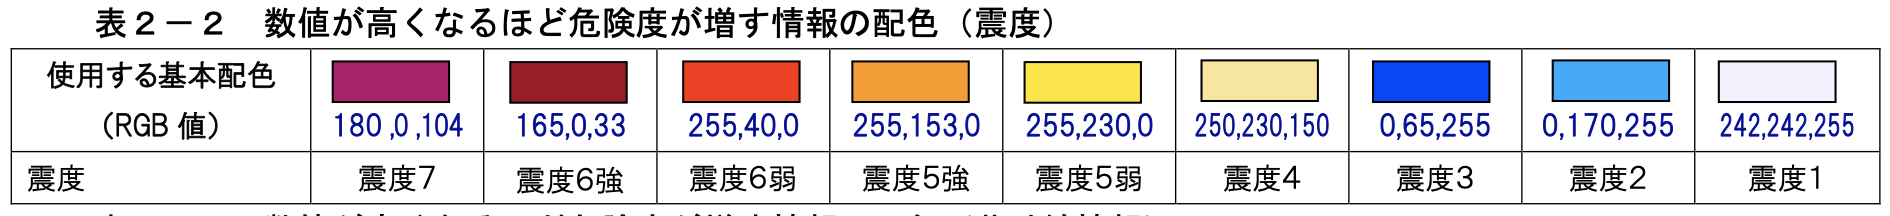
\includegraphics[width=0.8\linewidth]{jma-colour-scheme-intensity.png}
    \caption{JMA Colour Scheme for Measured Intensities}
    \label{fig:jma-colour-scheme-intensity}
\end{figure}

\begin{figure}[htp]
    \centering

    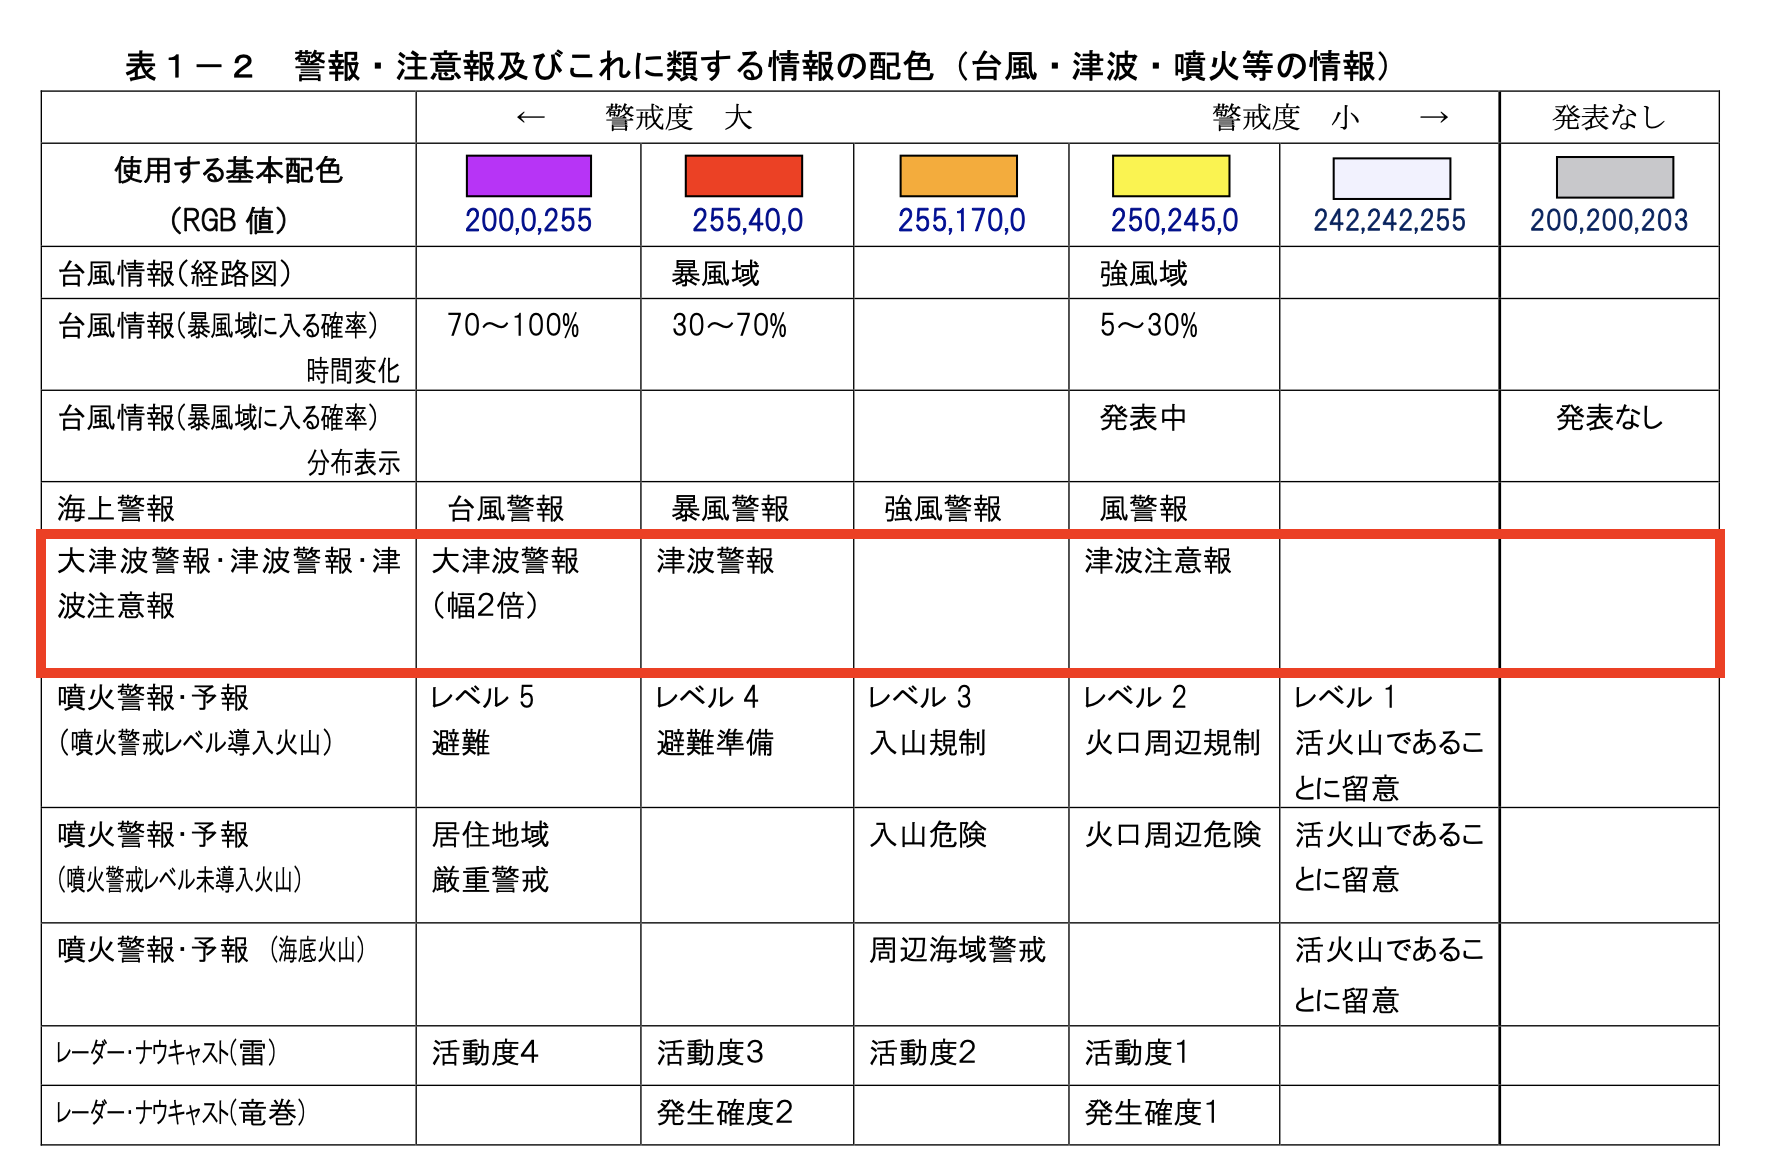
\includegraphics[width=0.8\linewidth]{jma-colour-scheme-tsunami.png}
    \caption[JMA Colour Scheme for Tsunamis]{JMA Colour Scheme for Tsunamis\\
        Purple: Special Warning; Red: Tsunami Warning; Yellow: Tsunami Caution}
    \label{fig:jma-colour-scheme-tsunami}
\end{figure}

In addition to these colours, for tsunami informational advisory, the colour \Colour{80FFFF} is used, in accordance with the colour used for no release of river flooding warning, and for endings of tsunamis warnings, the colour \Colour{F2F2FF} is used, in accordance with the minimal level (the extremely light grey) in \autoref{fig:jma-colour-scheme-tsunami}.

The colour \Colour{F0F0F0} is used for intensity zero (i.e. any intensity less than intensity 1), and \Colour{C8C8CB} is used for unknown intensities.

A similar colour scheme is used for EEW warnings. Specifically, the same colour as tsunami warning is used for EEW warnings, and the same colour as endings of tsunami warnings is used for EEW cancellation. For EEW forecasts, the colour \Colour{FFAA00} (in accordance with the orange colour in \autoref{fig:jma-colour-scheme-tsunami}) is used, and for EEW final reports, the same colour is used as unknown intensities.

A summary of the colours used is in the table below.

\begin{table}[htp]
    \centering
    \begin{tabular}{c|c}
        Intensity & Colour          \\
        \hline
        ?         & \Colour{C8C8CB} \\
        0         & \Colour{F0F0F0} \\
        1         & \Colour{F2F2FF} \\
        2         & \Colour{00AAFF} \\
        3         & \Colour{0041FF} \\
        4         & \Colour{FAE696} \\
        5-        & \Colour{FFE600} \\
        5+        & \Colour{FF9900} \\
        6-        & \Colour{FF2800} \\
        6+        & \Colour{A50021} \\
        7         & \Colour{B40068}
    \end{tabular}
    \begin{tabular}{c|c}
        EEW Level & Colour          \\
        \hline
        Forecast  & \Colour{FFAA00} \\
        Warning   & \Colour{FF2800} \\
        Final     & \Colour{C8C8CB} \\
        Cancelled & \Colour{F2F2FF}
    \end{tabular}
    \begin{tabular}{c|c}
        Tsunami Warning Level & Colour          \\
        \hline
        Information           & \Colour{80FFFF} \\
        Caution               & \Colour{FAF500} \\
        Warning               & \Colour{FF2800} \\
        Special Warning       & \Colour{C800FF} \\
        None                  & \Colour{F2F2FF}
    \end{tabular}
    \caption{Colour Scheme for Application}
    \label{tab:colour-scheme}
\end{table}

\subsection{Details to Display}
Comparing the information provided by the different applications, the following information about an earthquake will be displayed in the sidebar, as consistent with most applications analysed:
\begin{itemize}
    \item Maximum observed intensity of earthquake;
    \item Time of the earthquake;
    \item Name of position of hypocentre;
    \item Depth of hypocentre;
    \item Magnitude of the earthquake.
\end{itemize}

In addition to these, on the side panel, the following information will be displayed in addition to the previous ones:
\begin{itemize}
    \item Last updated time of information;
    \item The tree of intensities measured by observation stations, in hierarchy structure of:
          \begin{enumerate}
              \item Intensity; then by
              \item Prefecture; then by
              \item Regions; then by
              \item Cities/Districts; finally
              \item Observation Stations.
          \end{enumerate}
    \item Any additional text provided by the JMA on the report, where applicable.
\end{itemize}

Note there is an extra level of regions in the hierarchy tree, compared to KEVI.

As for the EEW warning, there are slightly different information displayed, due to different information provided, and the nature of the EEW. The following information will be displayed:
\begin{itemize}
    \item The level of the EEW warning;
    \item The serial number of the EEW warning,
    \item Maximum predicted intensity of earthquake;
    \item Origin time of the earthquake;
    \item Name of position of hypocentre;
    \item Warning text if the hypocentre is assumed (as a JMA requirement);
    \item Depth of hypocentre;
    \item Magnitude of the earthquake;
    \item Precision/Accuracy of information on hypocentre, depth and magnitude;
    \item Warning text if the earthquake has low accuracy (as a JMA requirement);
    \item Last updated time of the information,
    \item Any additional text provided by the JMA on the report, where applicable.
\end{itemize}

Note that (as a JMA requirement), if the hypocentre is assumed for algorithmic reasons, then the hypocentre details and the magnitude have no seismological meaning, and the information on origin time, the position of hypocentre, the depth of hypocentre and the magnitude of the earthquake will be hidden

The information displayed for a tsunami warning will be relatively simple:
\begin{itemize}
    \item The level of the tsunami warning;
    \item Any additional text provided by the JMA on the report, where applicable.
\end{itemize}